%% LyX 2.1.4 created this file.  For more info, see http://www.lyx.org/.
%% Do not edit unless you really know what you are doing.
\documentclass[12pt,english]{report}
\usepackage{charter}
\renewcommand{\familydefault}{\rmdefault}
\usepackage[T1]{fontenc}
\usepackage[a4paper]{geometry}
\geometry{verbose,tmargin=2.5cm,bmargin=2.5cm,rmargin=2.5cm}
\setcounter{secnumdepth}{3}
\setcounter{tocdepth}{3}
\setlength{\parskip}{\medskipamount}
\setlength{\parindent}{0pt}
\usepackage{color}
\usepackage{babel}
\makeatletter

\makeatother
\usepackage{float}
\usepackage{graphicx}
\usepackage{setspace}
\usepackage{nomencl}
% the following is useful when we have the old nomencl.sty package
\providecommand{\printnomenclature}{\printglossary}
\providecommand{\makenomenclature}{\makeglossary}
\makenomenclature
\onehalfspacing
\usepackage[unicode=true,
 bookmarks=true,bookmarksnumbered=true,bookmarksopen=true,bookmarksopenlevel=1,
 breaklinks=true,pdfborder={0 0 1},backref=false,colorlinks=true]
 {hyperref}
\hypersetup{
 linkcolor=black, citecolor=red, urlcolor=blue, filecolor=blue, pdfstartview=XYZ}

\makeatletter

%%%%%%%%%%%%%%%%%%%%%%%%%%%%%% LyX specific LaTeX commands.
%% Because html converters don't know tabularnewline
\providecommand{\tabularnewline}{\\}

%%%%%%%%%%%%%%%%%%%%%%%%%%%%%% User specified LaTeX commands.
% the pages of the TOC is numbered roman
% and a pdf-bookmark for the TOC is added
\pagenumbering{roman}

%\let\myTOC\tableofcontents
%\renewcommand\tableofcontents{%
 % \pdfbookmark[1]{\contentsname}{}
 % \myTOC
 % \cleardoublepage  }

%*****Chapter style******
\usepackage[Glenn]{fncychap}
\ChNameVar{\large}
\ChTitleAsIs
\ChTitleVar{\bfseries\Huge}

%*****Header style*******
\usepackage{fancyhdr}
 
\pagestyle{fancy}

\fancyhf{}
\fancyhead[LE,RO]{\thepage}
\fancyhead[RE,LO]{\footnotesize\nouppercase{\leftmark}}

%\renewcommand{\chaptermark}[1]{\markboth{#1}{}}

\renewcommand{\headrulewidth}{0,5pt}

%****Glossaire Title*****
\renewcommand{\nomname}{Glossaire}

\makeatother

\begin{document}
\noindent \begin{titlepage}
\begin{center}
% Upper part of the page
\begin{minipage}{0.4\textwidth}   Réf : xx/xx  \end{minipage}
\begin{minipage}{0.4\textwidth} \begin{flushright} A.U. : 2014-2015 \end{flushright}\end{minipage}
\rule[0.5ex]{1\columnwidth}{1pt}\\[0.5cm]
\textsc{\large{Université de Sousse}}\\
\textsc{\large{Ecole Nationale d'Ingénieurs de Sousse}}\\
%\includegraphics[width=0.3\textwidth]{logo.png}\\[-0.5cm]
\Large{Rapport de Projet de Fin d'Etudes}\\[0.5cm]
\normalsize{Présenté en vue de l'obtention du diplôme d'}\\
\Large{ \bfseries{Ingénieur en Génie .....}}\\
\normalsize{Option ...}\\[0.6cm]
\rule[0.5ex]{1\columnwidth}{1pt}\\[0.5cm]
{ \huge \bfseries Conception et développement d'une application }\\[0.5cm]
\rule[0.5ex]{1\columnwidth}{1pt}\\[2cm]
% Author and supervisor
\begin{minipage}{0.4\textwidth} \begin{flushleft} \large \emph{Réalisé par:}\\ Prénom~\textsc{Nom} \end{flushleft} \end{minipage} \begin{minipage}{0.5\textwidth} \begin{flushright} \large \emph{Encadré par:} \\  Mr.~Prénom~\textsc{Nom} \end{flushright} \end{minipage}
\vfill
% Bottom of the page 
\end{center}
\end{titlepage}


\newpage
~\\
~\\
~\\
~\\
\begin{center}
To my family and all my beloved.
\end{center}



\chapter*{Acknowledgements}

I would like to express my gratitude towards my university's supervisor, Mr. Taha Ben Salah, and my company's supervisor Mr. Richard Lindberg for supporting me during my internship and for all the knowledge and experience they shared with me.
I would also like to thank all my professors for teaching me and helping me achieve my goals.


\tableofcontents{}

\listoffigures


\listoftables



\chapter*{Abstract}
My graduation project consists in creating a web application that contains listings of hotels, restaurants and any place available in the Google places API and allows registered users to create reviews about these places as well as rate them following some specific criteria like the use of renewable energy and the use of recyclable materials...
The web app also provides a REST API that is being used by a mobile app developed separately. Part of the project also consists in deploying the app to the cloud.


\section*{Keywords}
Python - Django - Sustainable Tourism - REST API - Amazon Web Services - Ratings



\pagenumbering{arabic} 



\chapter{Context}
\section{Introduction}

The internet is full of tourism platforms that list hotels, restaurants and similar tourism related services. To name a few of them we can cite as notable examples: Tripadvisor, Trivago and Kayak. There is literally tens of these platforms, from different countries and in different shapes and colours. However all of the existing platforms only let users write "general" reviews about the listed places, and the visitors can only distinguish between those places based on either the prices or the "general" reviews.
It turns out that there's also a market for people who are interested in "sustainable tourism" and don't mind paying more for an eco-friendly vacation. Sustainable tourism is defined as "tourism that respects local people, the traveller, cultural heritage and the environment" by UNESCO\cite{UNESCO}, you think of it as "fairtrade" and "organic" but for the travel sector.

One Planet Rating (OPR) was created to fill this void and serve this portion of tourists by listing the same places while focusing on sustainability instead of price.
One Planet Rating is a newly founded social startup based in Stockholm, with a portion of its team members working remotely (partially including myself). The startup is in its very early stages, its main product/service is the web application described in this report.
The company thrives to have an impact and aims, with its services, to help achieve some of the United Nations' Sustainable Development Goals (UN SDGs)\cite{UN} like:
\begin{itemize}

\item UN SDG 8: "Promote sustained, inclusive and sustainable economic growth, full and productive employment and decent work for all".
\item UN SDG 15: Protect, restore and promote sustainable use of terrestrial ecosystems, sustainably manage forests, combat desertification, and halt and reverse land degradation and halt biodiversity loss"
\item UN SDG 13: "Take urgent action to combat climate change and its impacts by regulating emissions and promoting developments in renewable energy.
\end{itemize}
OPR is a tourism platform that is sustainability-focused, it allows people from around the world to rate and review touristic services based on how much they respect the earth.
The long term goal of OPR is to promote the movement of sustainable tourism and incite people to be more responsible during their trips, and eventually help protect the environment and the community.
OPR also emphasizes on transparency as it doesn't participate in writing the reviews and ratings, it only provides a playground for all people to express themselves freely.


In this report we briefly cover the state of the art and market analysis of the project.
In the first chapter we go through the requirements and specifications.
The second chapter covers the design aspects of the project.
The third chapter covers the development and deployment aspects of the project.


\section{State of the art}


Many online tourism platforms exist today, we can consider these platforms as "indirect competitors" because they offer an alternative functionality to OPR, but what makes the most difference is the target market.
Some of these major platforms are Tripadvisor (fig.\ref{fig:tripadvisor}), Trivago (fig.\ref{fig:trivago}) and Momondo(fig.\ref{fig:momondo}).
As shown in the following screenshots, all of those platforms focus on the general ratings and the price.
They offer very similar functionalities but in different layouts.

\begin{figure}[H]
\centering
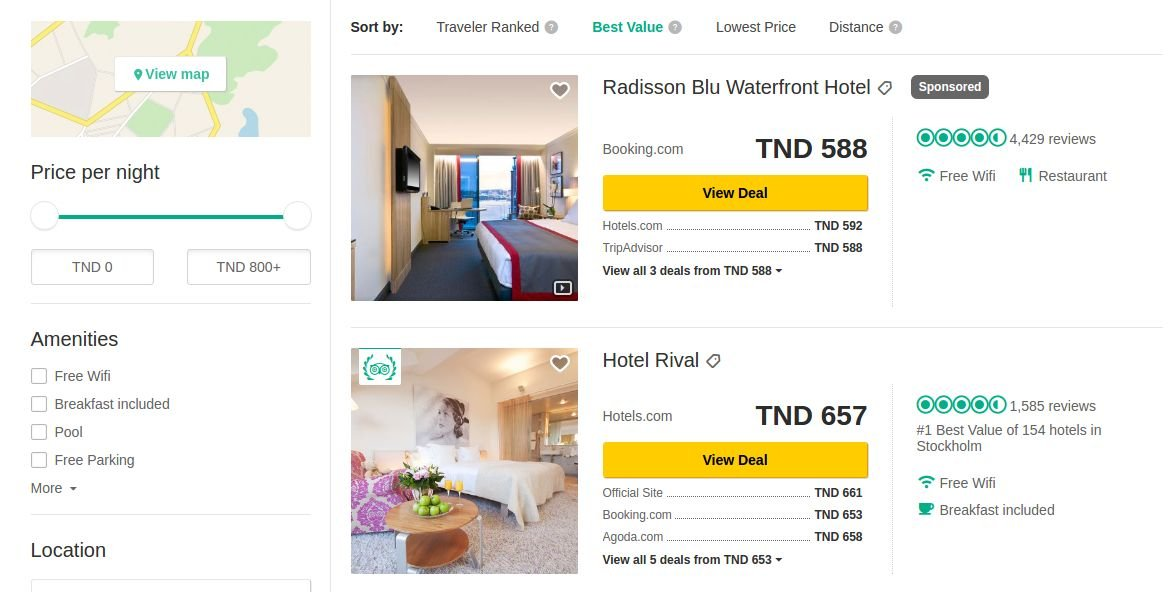
\includegraphics[width=15cm]{tripadvisor.jpg}
\caption{screenshot of Tripadvisor}
\label{fig:tripadvisor}
\end{figure}


Tripadvisor, which is the world leader in the tourism sector, provides hotel booking and listing of tourism establishments. The company is based in the United States and it also offers other related services like tourism focused forums. The platform also allows users to search for and book flight tickets.

\begin{figure}[H]
\centering
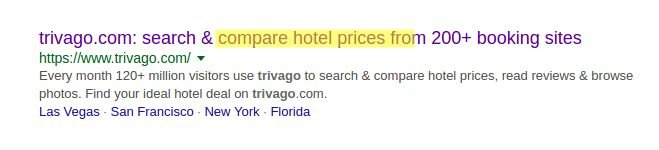
\includegraphics[width=15cm]{trivago.jpg}
\caption{screenshot of search results for Trivago}
\label{fig:trivago}
\end{figure}

In contrast, the Germany based company, Trivago, only focuses on hotels. Trivago is the leader hotel search engine in Germany\cite{PAOLO}. Though trivago only lists hotels, it is owned by Expedia, which owns and operates more than 200 websites that offer diverse services in the tourism and travel sectors.


\begin{figure}[H]
\centering
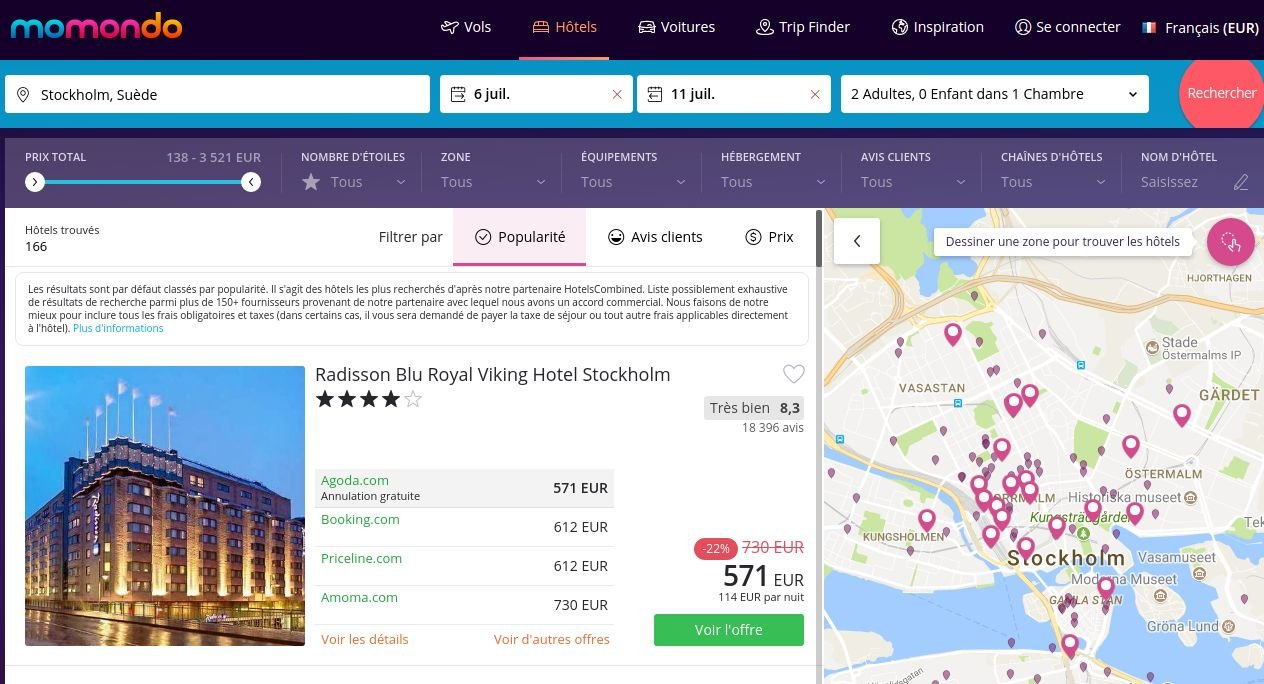
\includegraphics[width=15cm]{momondo.jpg}
\caption{screenshot of Momondo}
\label{fig:momondo}
\end{figure}

Momondo is also a similar service which, in addition to listing hotels, also provides flight booking and car rental services. Another interesting thing about Momondo is that it is based in Scandinavia, and this makes of it a local competitor.

Another thing to note is that most of these "indirect competitors" are booking websites while OPR is not. OPR's goal is to promote the sustainable places and discourage the unsustainable ones.





The following table shows more in detail the difference between OPR and the above-mentioned competitors:
\begin{table}[H]
\centering
\begin{tabular}{|l|l|l|l|l|}
\hline
Funtionality                       & Tripadvisor & Trivago & Momondo & OPR \\ \hline
Search hotels                      & YES         & YES     & YES     & YES \\ \hline
Search restaurants                 & YES         & NO      & NO      & YES \\ \hline
Search activities and other places & YES         & NO      & NO      & YES \\ \hline
Search for flights                 & YES         & NO      & YES     & NO  \\ \hline
Search for flights                 & NO          & NO      & YES     & NO  \\ \hline
Booking service                    & YES         & YES     & YES     & NO  \\ \hline
General ratings                    & YES         & YES     & YES     & YES \\ \hline
Sustainability ratings              & NO          & NO      & NO      & YES \\ \hline
\end{tabular}
\caption{comparison of tourism platforms}
\label{my-label}
\end{table}




Another category of competitors includes magazines, blogs and expert websites (fig.\ref{fig:blog}) that promote some specific sustainable places. Those are also indirect competitors because they rely on experts' advice on their reviews which tend to be not very trustworthy. OPR's content will be completely user generated, because most people believe more in reviews created by peers and want to be part of the content creation. OPR will only be the intermediary between content creators and content consumers, and will not participate in content creation.

\begin{figure}[H]
\centering
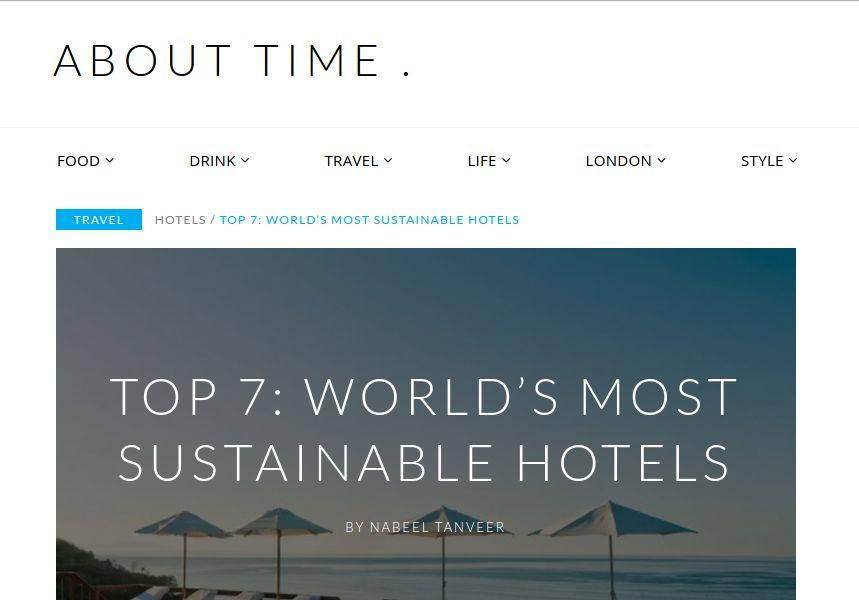
\includegraphics[width=15cm]{blog.jpg}
\caption{example of an expert blog}
\label{fig:blog}
\end{figure}


\section{Formalism}
During the work on this project we used the following formal methods:
\subsection*{UML}
We used UML (Unified Modeling Language)for describing and modeling the specifications of the project. UML is very flexible and versatile. UML is also one of the best choices for modeling because it is very popular and widely used across the globe, which makes it easier to grasp by other people. Most software engineers are probably familiar with it.
\subsection*{Agile scrum}
We used the agile scrum method because it is the most convenient method to the project. Every week we have a sprint where we define the goals of that week from the backlog. This methodology turned to be very efficient, especially that the project consists in developing a prototype, which requires continuous thinking and customization. Agile scrum allowed us to customize the project while working on it.


\chapter{Specifications}
\section{Actors}
\subsection{Internal actors}
\paragraph{User}
~\\
Anybody who accesses OPR Ratings via App or Web is a User. As opposed to "Member" (see
below) this does not require any log-on, or creation of a OPR Profile.
A User can search for specific places and read reviews of those places.


\paragraph{Member}
~\\
OPR Members are Users who sign up to use OPR's services with a Profile. A User needs to be
logged in, to be acting as a Member.
A member can do everything a User can do, in addition to the ability of posting their own
reviews and ratings.

\paragraph{Manager}
~\\
In addition to the permissions that a Member has, an Admin has the permission to Create,
Read, Update and Delete (CRUD) Ads, reviews and rating categories.

\paragraph{Admin}
~\\
The admin is responsible of managing the users, he has the permission to CRUD users.


\subsection{External actors}


\paragraph{Google places service}
~\\
Google places API is a passive actor that is called for every search to look for relevant places based on provided location.\\
The API provides us with :\\
Basic information (Name, address..), Photo, Google's place\_id (unique identifier)

\paragraph{Google maps service}
~\\
Google Maps API is another passive actor that provides us with a map pointing at the specific location based on the location's place\_id we retrieve from Google Places API


\paragraph{Gmail service}
~\\
Google's Gmail is used to send the emails to users. This actor is also passive.


\section{Functionalities' overview}

The main functionality of the platform is to allow members to read and post reviews and ratings
about some specific places. Obviously this implies that they need to be able to register and login
to the platform. Users should also be able to search for a specific place by a keyword. And since
OPR is all about sustainability-related reviews, the platform offers the possibility to rate
establishments based on multiple criteria.
The platform also has a mobile app, and this implies that the web based app should provide an
API to supply the mobile app with the data.

\begin{figure}[H]
\centering
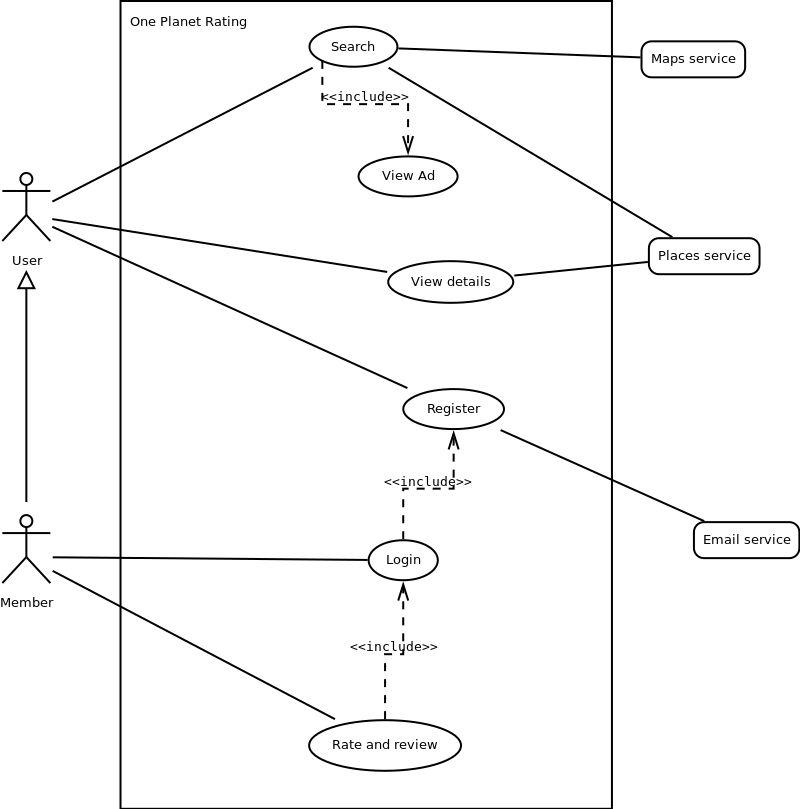
\includegraphics[width=15cm]{generalUseCase.jpg}
\caption{general usecase diagram}
\label{fig:generalusecase}
\end{figure}

As shown in the use case diagram (fig.\ref{fig:generalusecase}), any user can use the app to search and view the details of a
place. The search functionality pulls data from Google places service, and shows a map using
Google maps service.
When a user registers, he becomes a member. During the registration process Gmail service is
used to send a confirmation email.
The member can then login to his profile and becomes able to rate and review places.

\subsection{Register}

\begin{figure}[H]
\centering
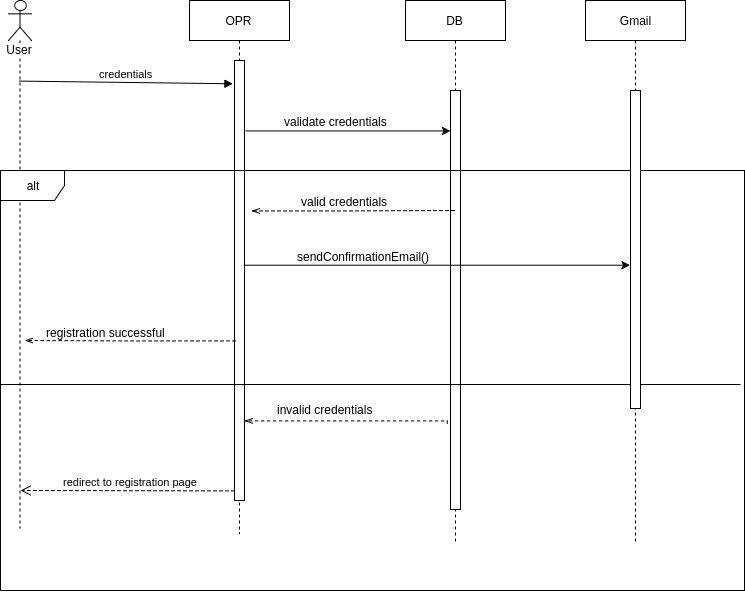
\includegraphics[width=15cm]{registerSequence.jpg}
\caption{registration sequence diagram}
\label{fig:registration}
\end{figure}

\begin{table}[H]
\centering
\begin{tabular}{|l|l|}
\hline
Title             & Registration                                                                                                                                                                                                                                                                                    \\ \hline
Author            & Moetaz Ben Charrada                                                                                                                                                                                                                                                                             \\ \hline
Version           & 1.0                                                                                                                                                                                                                                                                                             \\ \hline
Objectives        & Allows users to register and create an account                                                                                                                                                                                                                                                  \\ \hline
Actors            & User - OPR - Gmail                                                                                                                                                                                                                                                                              \\ \hline
Pre-conditions    & \begin{tabular}[c]{@{}l@{}}The user should be on the registration page\\ The user must not be already registered.\end{tabular}                                                                                                                                                                  \\ \hline
Post-conditions   & The user becomes registered (member)                                                                                                                                                                                                                                                            \\ \hline
Story             & \begin{tabular}[c]{@{}l@{}}1. The user enters his username\\ 2. The user enters his email\\ 3. The user enters his password\\ 4. The user re-enters his password\\ 5. The user submits the form\end{tabular}                                                                                    \\ \hline
Alternative story & \begin{tabular}[c]{@{}l@{}}The functionality is accessed through the\\ mobile app instead of a browser.\end{tabular}                                                                                                                                                                            \\ \hline
Exceptional story & \begin{tabular}[c]{@{}l@{}}If the user enters an email that's already in the DB,\\  the user will be prompted to enter a different email.\\ If the user enters a password that's not \\ compliant to the security constraints, he will\\ be prompted to enter a different password\end{tabular} \\ \hline
\end{tabular}
\caption{Registration description}
\label{my-label}
\end{table}


Every user can register (fig.\ref{fig:registration}) to OPR and becomes a member. A member has the option to post reviews in addition to all the privileges a normal use has. The registration process starts by the user entering his username, email and password. After submitting these information, OPR's registration system checks the unicity of the email and username, as well as the strength of the password. If either the username or email are not unique, or the password is not secure enough (i.e. at least 8 characters, composed of letters, numbers and special characters), the user will be prompted to re-enter the data with changes to the fields in question.\\When the data is valid, OPR sends an email-confirmation request to the new member. OPR sends the email via Gmail, through an SMTP connection. A registration is only considered complete after the email verification occurs.

\subsection{Login}

\begin{figure}[H]
\centering
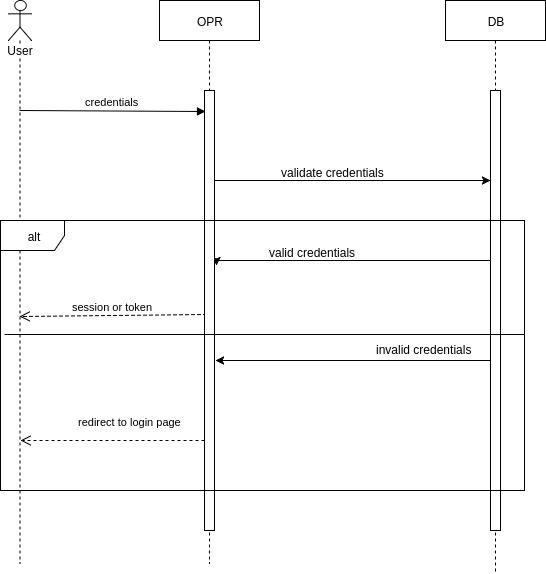
\includegraphics[width=15cm]{loginSequence.jpg}
\caption{login sequence diagram}
\label{fig:login}
\end{figure}

\begin{table}[H]
\centering
\begin{tabular}{|l|l|}
\hline
Title             & Login                                                                                                                                      \\ \hline
Author            & Moetaz Ben Charrada                                                                                                                        \\ \hline
Version           & 1.0                                                                                                                                        \\ \hline
Objectives        & Allows users to login and access his account                                                                                               \\ \hline
Actors            & User - OPR                                                                                                                                 \\ \hline
Pre-conditions    & \begin{tabular}[c]{@{}l@{}}The user should be a registered member.\\ The user must not be already logged in.\end{tabular}                  \\ \hline
Post-conditions   & \begin{tabular}[c]{@{}l@{}}The user becomes authenticated.\\ The user can then post reviews.\end{tabular}                                  \\ \hline
Story             & \begin{tabular}[c]{@{}l@{}}1. The user enters his username\\ 2. The user enters his password\\ 3. The user submits the form\end{tabular}   \\ \hline
Alternative story & \begin{tabular}[c]{@{}l@{}}The functionality is accessed through the\\ mobile app instead of a browser.\\ (Through the REST API)\end{tabular} \\ \hline
Exceptional story & \begin{tabular}[c]{@{}l@{}}If the user enters incorrect credentials, he will\\ be prompted to try to login again.\end{tabular}             \\ \hline
\end{tabular}
\caption{login description}
\label{my-label}
\end{table}

Another basic functionality of the app is letting users log in (fig.\ref{fig:login}). In fact users need to log in to be able to post reviews. And to be able to login, the user must be already registered. To login, the user provides his username and password. If they are valid the user is either given a cookie (if he is using a web browser) or an authentication token (if he is using the mobile app). If the credentials he provided are invalid he is prompted to try to log in again.


\subsection{Search}



\begin{figure}[H]
\centering
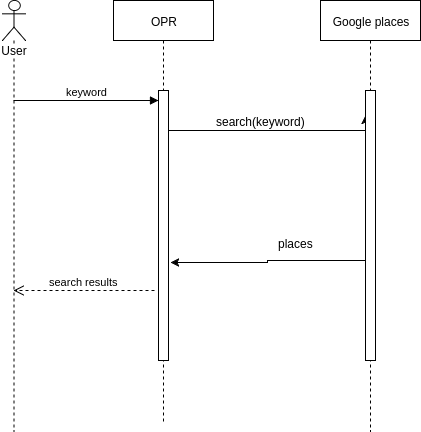
\includegraphics[width=12cm]{searchSpec.png}
\caption{search sequence diagram}
\label{fig:search}
\end{figure}


\begin{table}[H]
\centering
\begin{tabular}{|l|l|}
\hline
Title             & Search                                                                                                                                                                              \\ \hline
Author            & Moetaz Ben Charrada                                                                                                                                                                 \\ \hline
Version           & 1.0                                                                                                                                                                                 \\ \hline
Objectives        & Allows users to search for a specific place.                                                                                                                                        \\ \hline
Actors            & User - OPR - Places service                                                                                                                                                         \\ \hline
Pre-conditions    & \begin{tabular}[c]{@{}l@{}}The user should be on a page where there's\\ a search bar.\end{tabular}                                                                                  \\ \hline
Post-conditions   & \begin{tabular}[c]{@{}l@{}}The user finds places related to his keywords,\\ and may click to check the details of that\\ place.\end{tabular}                                        \\ \hline
Story             & \begin{tabular}[c]{@{}l@{}}1. The user enters keywords related \\ to the place he's looking for\\ 2. The user selects the type of place\\ 3. The user submits the form\end{tabular} \\ \hline
Alternative story & \begin{tabular}[c]{@{}l@{}}The functionality is accessed through the\\mobile app instead of a browser.\\ (Through the REST API)\end{tabular}                                          \\ \hline
\end{tabular}
\caption{search description}
\label{my-label}
\end{table}

The search functionality (fig.\ref{fig:search}) is a basic but essential functionality of the app. It allows the user to look for a location based on its type (Hotel, restaurant, activity) and location. The search bar offers autocomplete functionality to assist the user with the location names. After a user submits a search query, OPR will make HTTP calls to google's places services to find the locations. The response from the call is formatted, and OPR's data is added (average rating + number of reviews) and then delivered to the client.

\subsection{View details}


\begin{figure}[H]
\centering
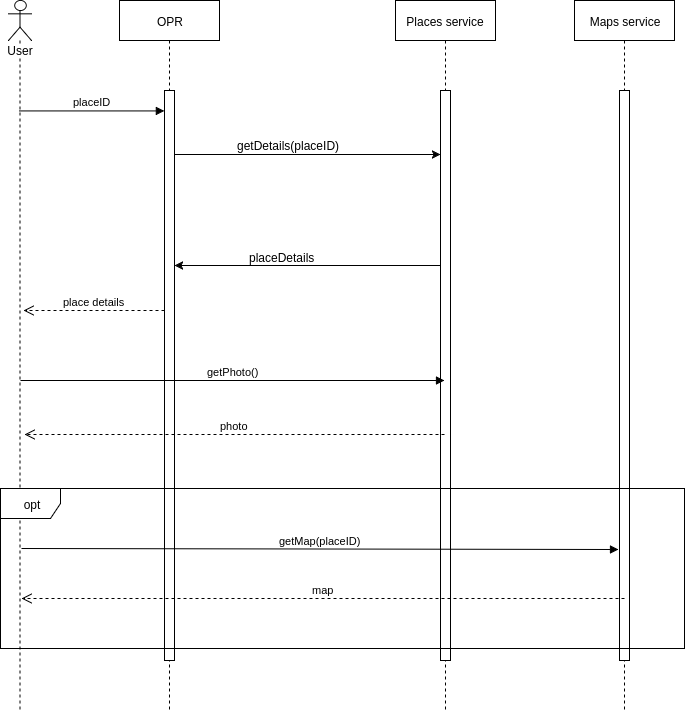
\includegraphics[width=15cm]{viewSpec.png}
\caption{view details sequence diagram}
\label{fig:details}
\end{figure}



\begin{table}[H]
\centering
\begin{tabular}{|l|l|}
\hline
Title             & View details                                                                                                                                                                                                                                                                                                                       \\ \hline
Author            & Moetaz Ben Charrada                                                                                                                                                                                                                                                                                                                \\ \hline
Version           & 1.0                                                                                                                                                                                                                                                                                                                                \\ \hline
Objectives        & \begin{tabular}[c]{@{}l@{}}Allows users to view the details and reviews\\ of a specific place\end{tabular}                                                                                                                                                                                                                         \\ \hline
Actors            & User - OPR - Places service - Maps service                                                                                                                                                                                                                                                                                         \\ \hline
Pre-conditions    & \begin{tabular}[c]{@{}l@{}}The user should have searched for the\\ place before.\end{tabular}                                                                                                                                                                                                                                      \\ \hline
Post-conditions   & \begin{tabular}[c]{@{}l@{}}The user sees the details and reviews of \\ the place and can possibly post a review about it.\end{tabular}                                                                                                                                                                                             \\ \hline
Story             & \begin{tabular}[c]{@{}l@{}}1. The user clicks on one of the places he found\\ in the search view.\\ 2. OPR app will then get the details of that\\  place from Google places service, get\\  the map from Google maps service.\\ 3. The data is combined with the local\\ reviews' data and is sent back to the user.\end{tabular} \\ \hline
Alternative story & \begin{tabular}[c]{@{}l@{}}The functionality is accessed through the\\ mobile app instead of a browser.\\ (Through the REST API)\end{tabular}                                                                                                                                                                                      \\ \hline
\end{tabular}
\caption{view-details description}
\label{my-label}
\end{table}

After searching for a place, the user will select one of the places shown in the search results, the user is then redirected to the view-details (fig.\ref{fig:details}) page. When the user does so, OPR calls Google's places service again, but this time to request the details of a specific place. The places are identified by their place\_id.

\subsection{Review a place}


\begin{figure}[H]
\centering
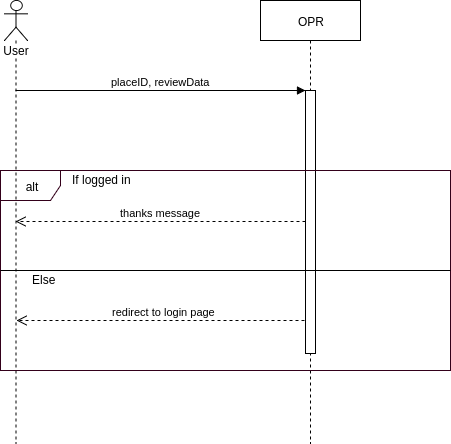
\includegraphics[width=13cm]{reviewSpec.png}
\caption{review a place sequence diagram}
\label{fig:review}
\end{figure}



\begin{table}[H]
\centering
\begin{tabular}{|l|l|}
\hline
Title             & Review a place                                                                                                                                                                                           \\ \hline
Author            & Moetaz Ben Charrada                                                                                                                                                                                      \\ \hline
Version           & 1.0                                                                                                                                                                                                      \\ \hline
Objectives        & \begin{tabular}[c]{@{}l@{}}Allows users to post a review about a specific\\ place\end{tabular}                                                                                                           \\ \hline
Actors            & User - OPR                                                                                                                                                                                               \\ \hline
Pre-conditions    & \begin{tabular}[c]{@{}l@{}}The user should be authenticated to be able\\ to post a review.\end{tabular}                                                                                                  \\ \hline
Post-conditions   & \begin{tabular}[c]{@{}l@{}}The user creates a review.\\ The review becomes visible to the public.\end{tabular}                                                                                           \\ \hline
Story             & \begin{tabular}[c]{@{}l@{}}1.The user enters his review data \\ 2.The user submits the form. \\ 3.The review data is saved to the \\ database.\\ 4.A thanks message is shown to\\ the user.\end{tabular} \\ \hline
Alternative story & \begin{tabular}[c]{@{}l@{}}The functionality is accessed through the\\ mobile app instead of a browser.\\ (Through the REST API)\end{tabular}                                                            \\ \hline
Exceptional story & \begin{tabular}[c]{@{}l@{}}If the user tries to post a review while\\  he's not authenticated. He is \\ redirected to the login page.\end{tabular}                                                       \\ \hline
\end{tabular}
\caption{review a place description}
\label{my-label}
\end{table}

After a user finds the place he is looking for, he can review (fig.\ref{fig:review}) that place. If he is not logged in, he is redirected to the login page. In case he is already logged in, the user is provided with a review form where he can enter his comments about the place as well as stars-based ratings following some specific criteria. After the user fills and submits the review form, the review is persisted in OPR's DB and the user is shown a thanks screen.

\begin{figure}[H]
\centering
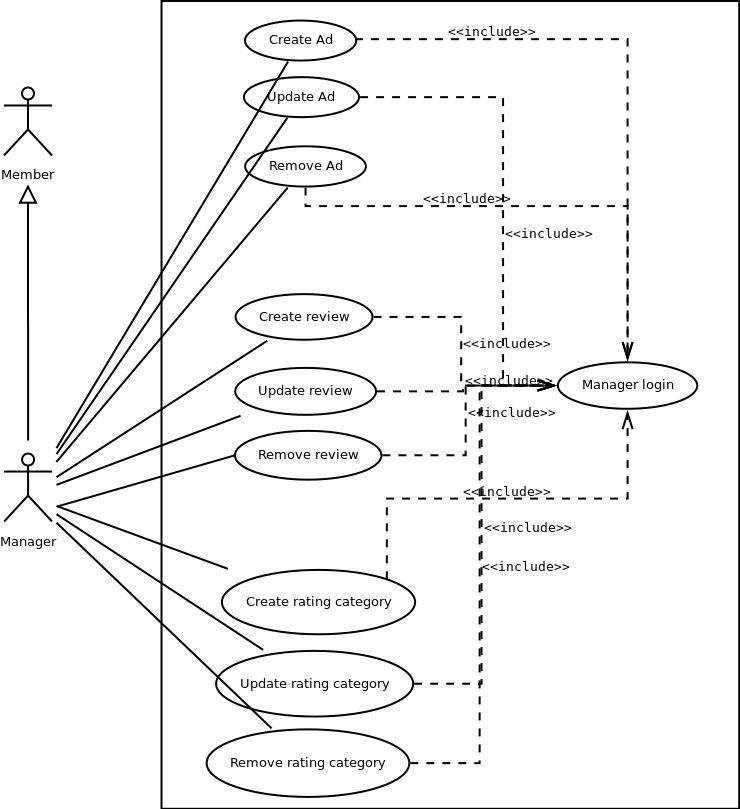
\includegraphics[width=15cm]{managerUseCase.jpg}
\caption{manager usecase diagram}
\label{fig:manager}
\end{figure}

A manager (fig.\ref{fig:manager}), is a member with additional privileges. A manager can create, update and delete:
ads, reviews and rating-categories.


\begin{figure}[H]
\centering
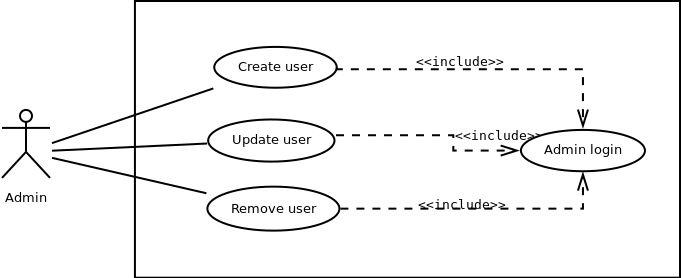
\includegraphics[width=15cm]{adminUseCase.jpg}
\caption{admin usecase diagram}
\label{fig:admin}
\end{figure}

The admin (fig.\ref{fig:admin}) however is only responsible for managing users. The admin can give and remove users' privileges, and thus can turn normal members into managers and vice-versa.

\chapter{Design \& architecture}
In this chapter we go through the design of the app from the ground up.
Since we are building the app from scratch we had to take into consideration both the physical and logical aspects of the app.\\~\\
As for the physical architecture, the app is designed in a way that prioritizes security and makes it easily scalable.\\~\\
In the logical side, the app is broken into smaller modules to facilitate maintainability and extensibility. During the design I aimed to make the modules independent to reduce coupling as much as possible, thus offering the possibility to easily change a module in the future, without touching the other modules.
\section{Physical architecture}
The main parts of our physical architecture (fig.\ref{fig:physicalarch}) are: The server hosting the web server and static files, the server hosting the app and the business logic and The DB server.\\~\\
For both the web server and the app server, we used an amazon EC2 instance running Ubuntu 16.04LTS.
AWS offers great support and scalability features.\\
The first server hosts the static files of the app (Images, CSS, JS) as well as the web server, in our case NGINX. The web server is configured to listen for the incoming requests, whether from a web browser or the mobile app. If the call is requesting a static file, NGINX will get the file using filesystem access and will send it back to the client. If the call is requesting a function to be run in the app, NGINX acts as a proxy\cite{JUSTIN} and redirects the call to the app server via HTTP, then gets the response and redirects it to the client.\\~\\
The second server is hosting the app, and the app server. Our app server is Gunicorn, it's a python WSGI server. That is where all the business logic is hosted and run. When a call only requires computing capabilities, this server will respond without needing any third parties. When the call requires external data, this server is responsible for acquiring that data.\\~\\
Our sources of data are either Google's APIs or our own DB. If the data needed is from Google, the app just triggers an HTTP request to Google's API.\\
If, on the other hand, the data requested is on our DB, the app has to access the DB through a TCP connection and get that data. The DB server is an AWS RDS instance hosting a PostgreSQL DB.
\begin{figure}[H]
\centering
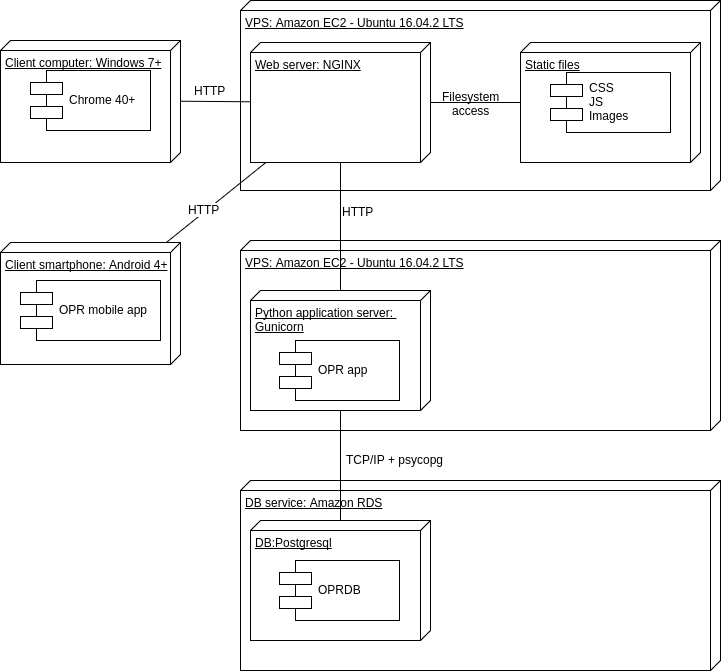
\includegraphics[width=15cm]{physicalArchitecture.png}
\caption{The app's physical architecture}
\label{fig:physicalarch}
\end{figure}

\section{Logical architecture}

The architecture (fig.\ref{fig:logicalarch}) used is a mix of MVC + 3 Tiers.

\paragraph{3 Tiers}
~\\
3 Tiers was used to separate the data, logic and the client from each other. Each of those three
tiers is a separate, standalone entity. This provides more security, because if one of the tiers
gets attacked the other tiers remain intact. This also provides some sort of interoperability
because we can change one of the tiers without touching the other ones.

\paragraph{MVC}
~\\
MVC architecture was used at the server level. MVC architecture facilitates code visibility and
maintainability because the architecture is well known and one can easily predict and
understand the functionality of each of its components. MVC also has the advantage of loose
coupling, which also offers interoperability as explained in the example of 3 Tiers above.


\begin{figure}[H]
\centering
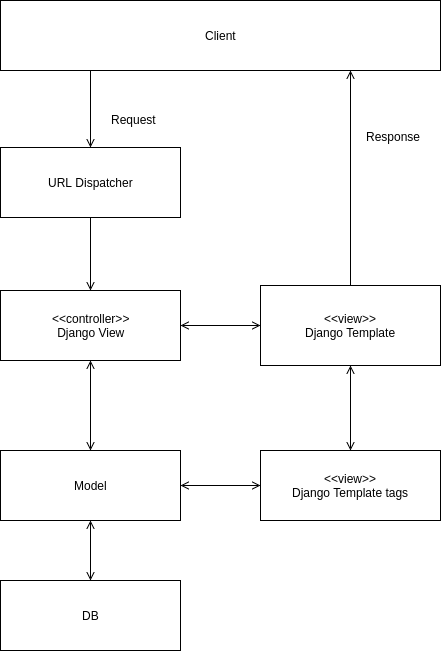
\includegraphics[width=12cm]{logicalArchitecture.png}
\caption{The app's logical architecture}
\label{fig:logicalarch}
\end{figure}


\section{Modular architecture}

\begin{figure}[H]
\centering
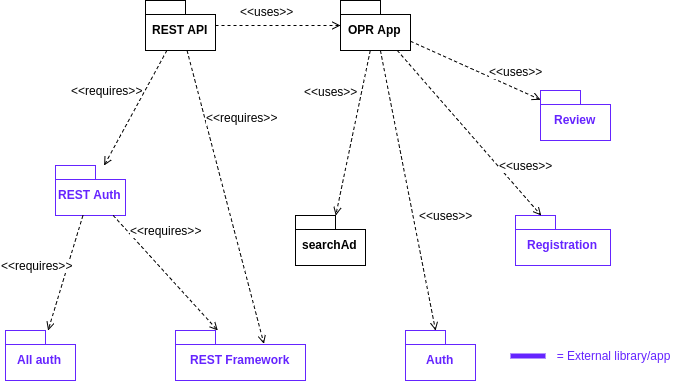
\includegraphics[width=15cm]{modularArchitecture.png}
\caption{The app's modular architecture}
\label{fig:modulararch}
\end{figure}

During my work on the project I tried my best to reuse existing code, thus some of the modules shown in the diagram (fig.\ref{fig:modulararch}) are external
libraries.
My work consists of creating the following modules:
OPR App, REST API and searchAd.

\section{Modules}

\subsection{searchAdModule}
This is a standalone library that offers the possibility to create and show ads either from a local
source (the user's DB) or from an external source (like Google Adsense).



\begin{figure}[H]
\centering
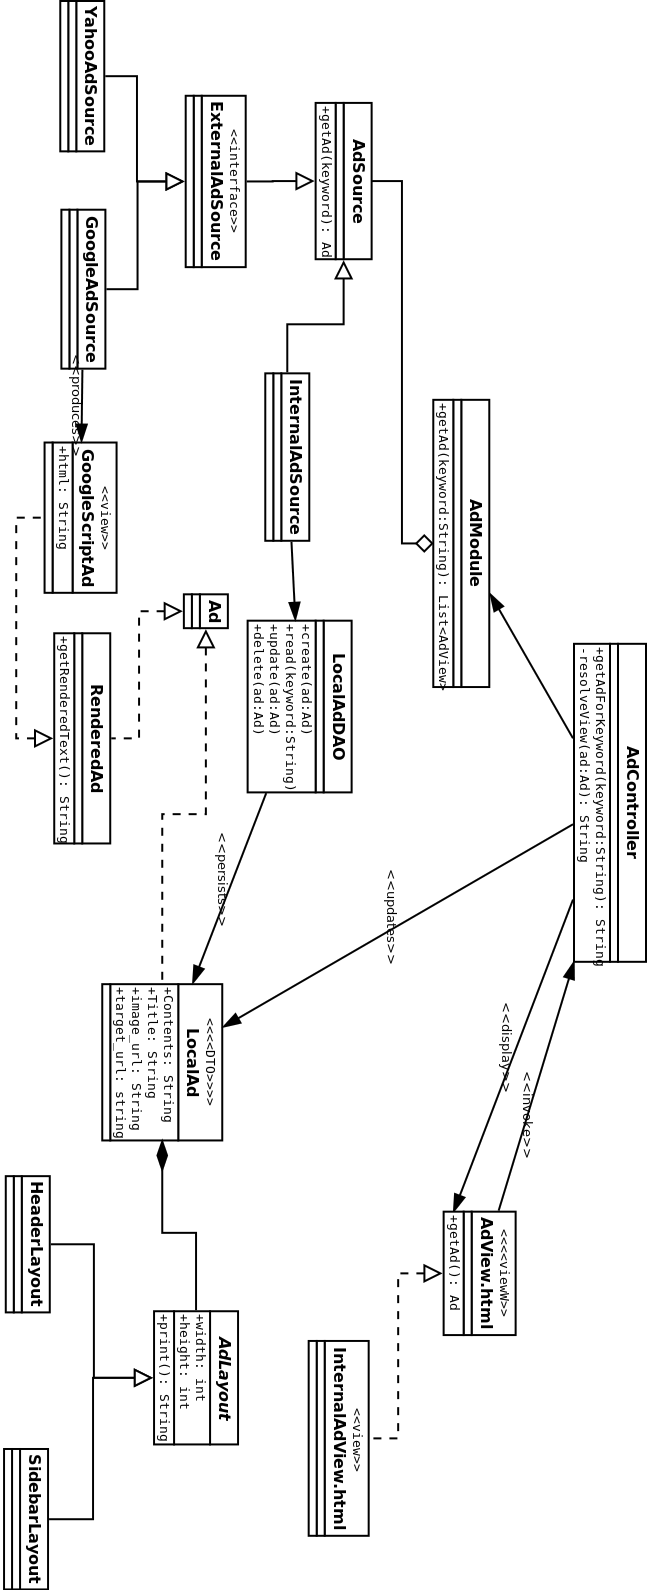
\includegraphics[width=10cm]{searchAdClass.png}
\caption{searchAd class diagram}
\label{fig:searchad}
\end{figure}

The searchAd module (fig.\ref{fig:searchad}) is designed following the MVC architecture.
The AdController is the entrypoint for the module, it allows the user to get an ad based on a
keyword. It also contains a private method resolveView() that shows the ad in html format to be
directly injected in the view.\\
The ExternalAdSource allows to get ads from external sources like Google AdWords. It is made
in a way to make it easily extensible with other external sources. In fact all we have to do is
create a new class inheriting the ExternalAdSource class and containing the url to the ads
service.\\
In case the ads are not pulled from an external source, they are stored in the local database as
LocalAd. The LocalAd model contains a title, content, target\_url and image\_url.


\subsection{OPR app module}
this is the main app, it contains the business logic for searching and rating places. It is also
where most of the other libraries are integrated and linked together.

\paragraph{Search}~\\

\begin{figure}[H]
\centering
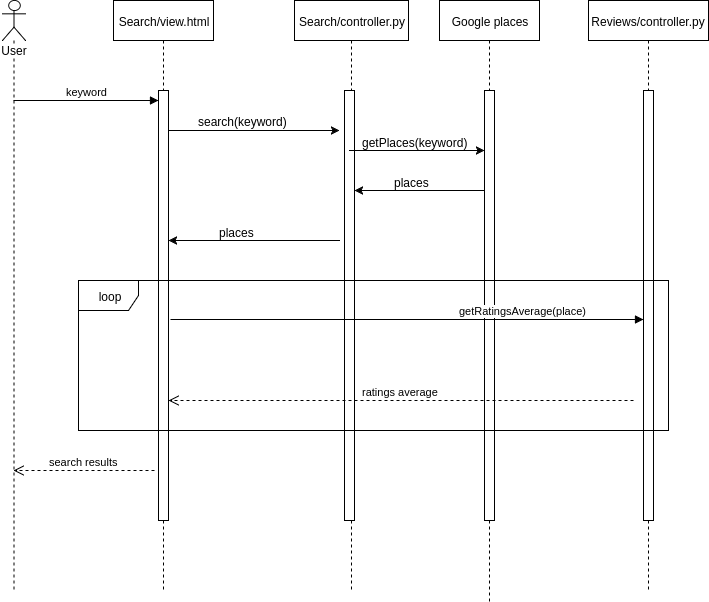
\includegraphics[width=15cm]{searchSequence.png}
\caption{search sequence diagram}
\label{fig:searchseq}
\end{figure}

When the user submits a keyword to search for, the search view (fig.\ref{fig:searchseq}) which is the intermediary between the user and the business logic gets the keyword and triggers the controller to process it. The search controller pulls the search results from Google places API and returns them to the view. The view also triggers the reviews controller to get the average ratings of the relevant places. The page returned to the user contains the places with their average ratings.


\paragraph{View details}~\\

\begin{figure}[H]
\centering
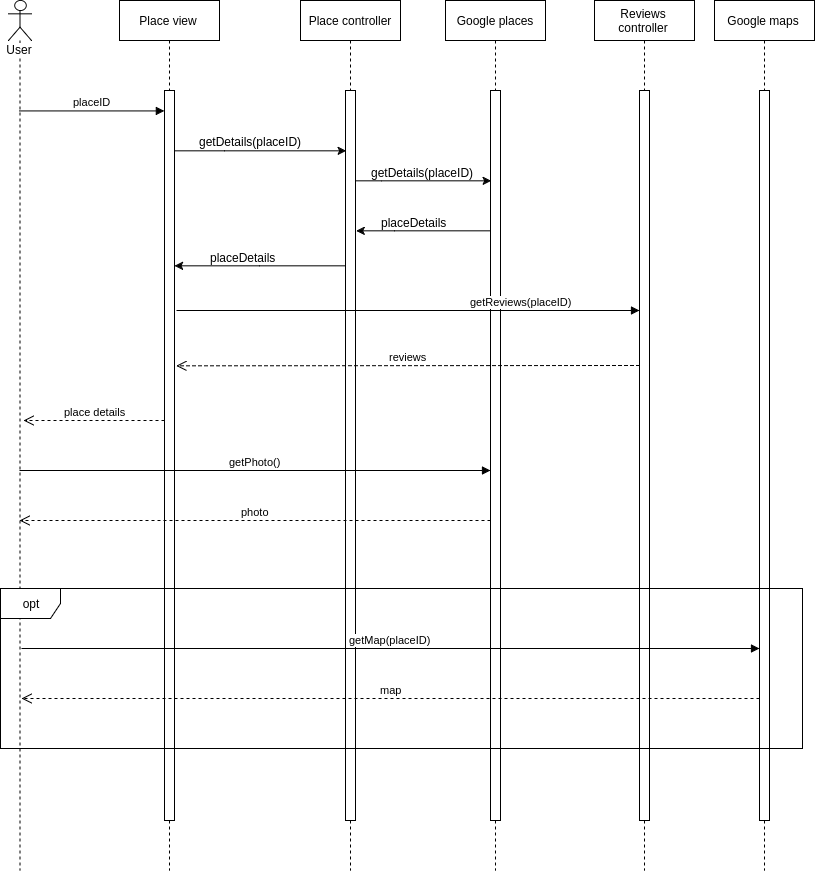
\includegraphics[width=15cm]{viewSequence.png}
\caption{view-details sequence diagram}
\label{fig:viewseq}
\end{figure}

When a user requests the details of a place (fig.\ref{fig:viewseq}), the place view triggers the place controller to get the details. Again the place controller pulls the data from Google places and returns them to the view. The view also gets the reviews from the reviews controller, and embeds the urls to the photo in the view. The view returned to the user contains the details, reviews and photo url of the place. Optionally the user may also want to see the map which is requested directly from Google maps by the browser.


\paragraph{Review a place}~\\

\begin{figure}[H]
\centering
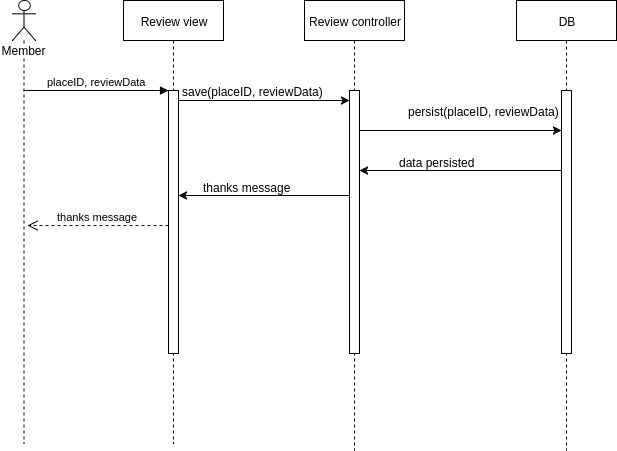
\includegraphics[width=15cm]{reviewSequence.png}
\caption{review a place sequence diagram}
\label{fig:reviewseq}
\end{figure}



Note that a user can only post a review (fig.\ref{fig:reviewseq}) if he is logged in. The process is explained in the
following interaction diagram (fig.\ref{fig:interaction})


\begin{figure}[H]
\centering
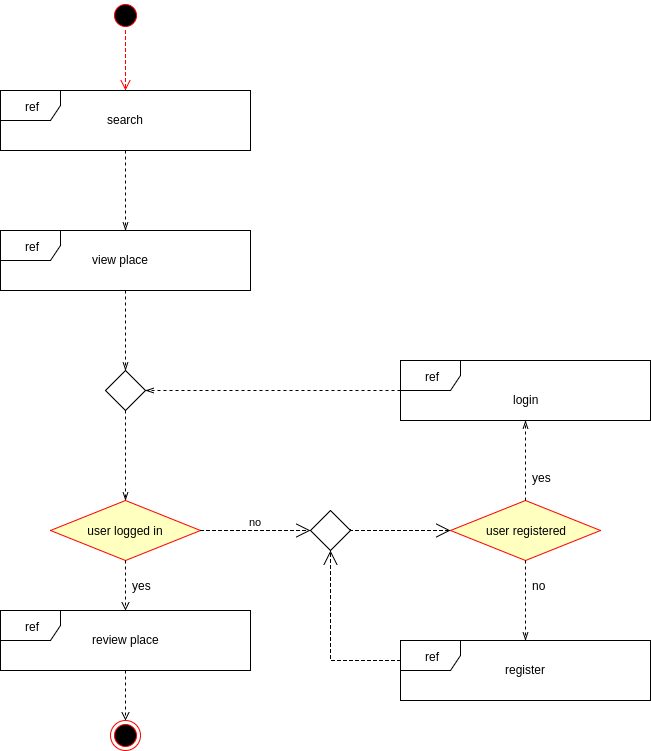
\includegraphics[width=15cm]{interactionDiagram.png}
\caption{interaction overview diagram}
\label{fig:interaction}
\end{figure}



\subsection{REST API module}
This is a sort of a wrapper for OPR App that provides a REST API interface, to be used by the mobile app.
\\For the REST API Module, I worked using the backwards approach\cite{WERNER}; I started by writing the user manual and documentation of the functionalities before implementing.\\



The services provided by the API are:
\begin{itemize}

\item Login
\item Register
\item Logout
\item Search for places
\item Get place details
\item Get reviews
\item Add review
\end{itemize}
The functions that require the transfer of critical data were designed to use the HTTP POST
method because it is more secure and it is the standard for this type of operations, for instance
we used POST for the authentication and registration functions. We also chose HTTP POST for
posting reviews, because it contains the authentication token, which is critical data, and it
contains the review's text, whose size might exceed the GET data size limit.\\
As for the other functionalities we used HTTP GET methods. One of the benefits of using GET
here is that you can share and bookmark links easier when the data is included in the URL.

\paragraph{Login}~\\
Authenticate the user with the system and obtain the auth\_token

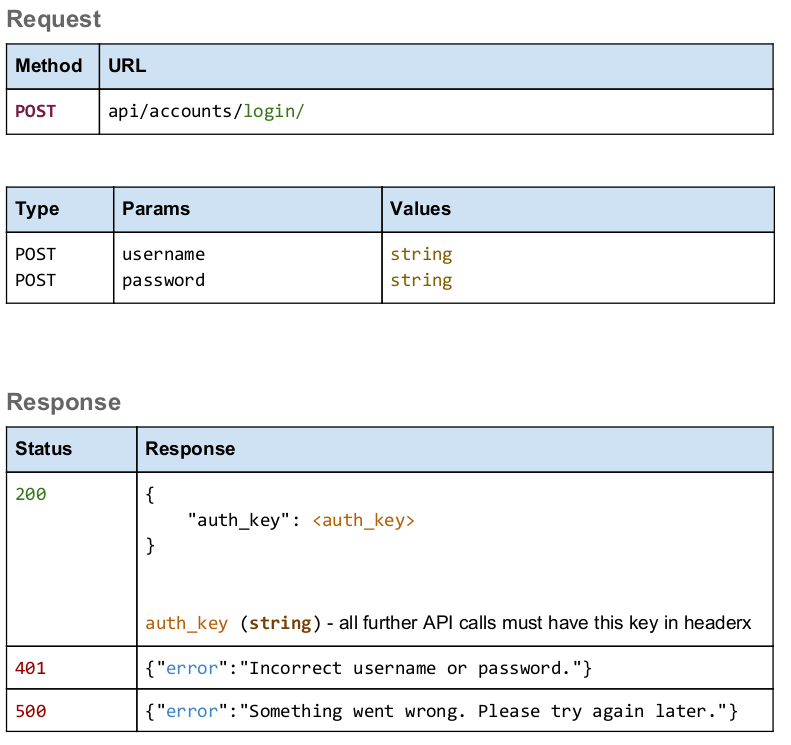
\includegraphics[width=15cm]{loginDoc.png}


\paragraph{Register}~\\
Create and add a new user to the app

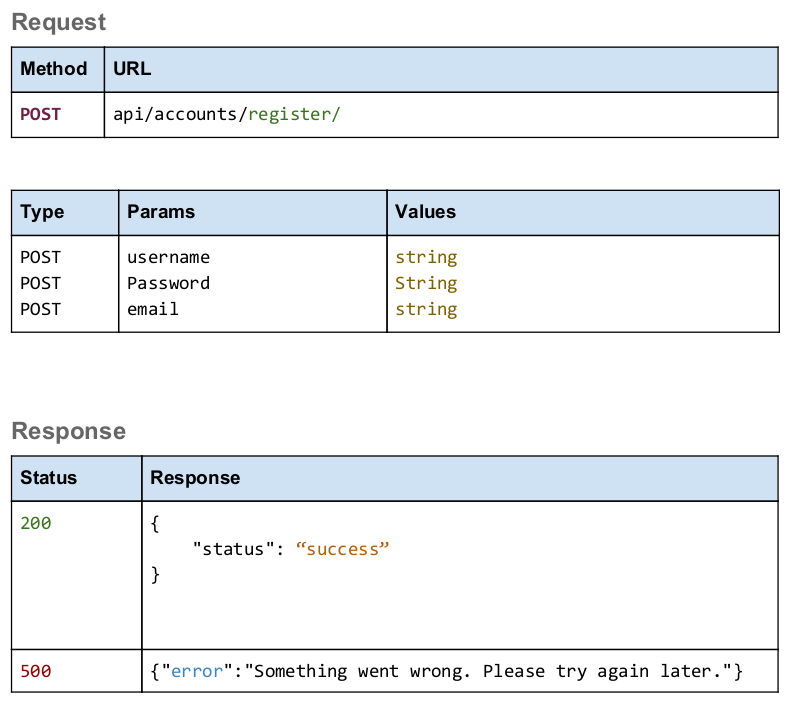
\includegraphics[width=15cm]{registerDoc.png}


\paragraph{Logout}~\\
Log out the current user

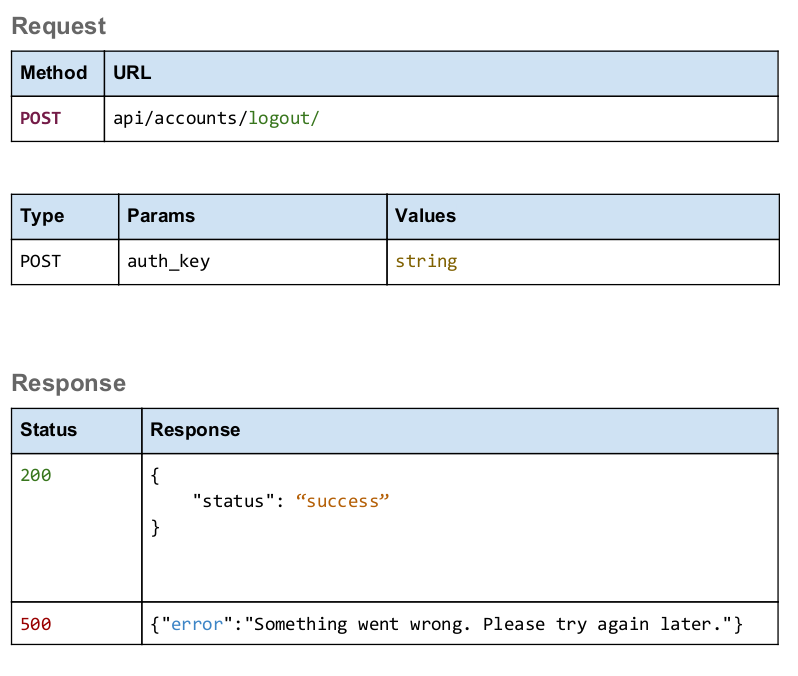
\includegraphics[width=15cm]{logoutDoc.png}


\paragraph{Search for places}~\\
Search for hotels, restaurants or activities

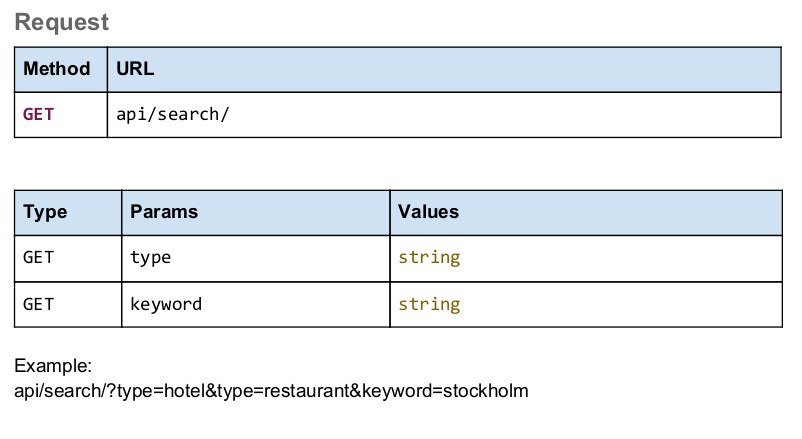
\includegraphics[width=15cm]{searchDoc.png}

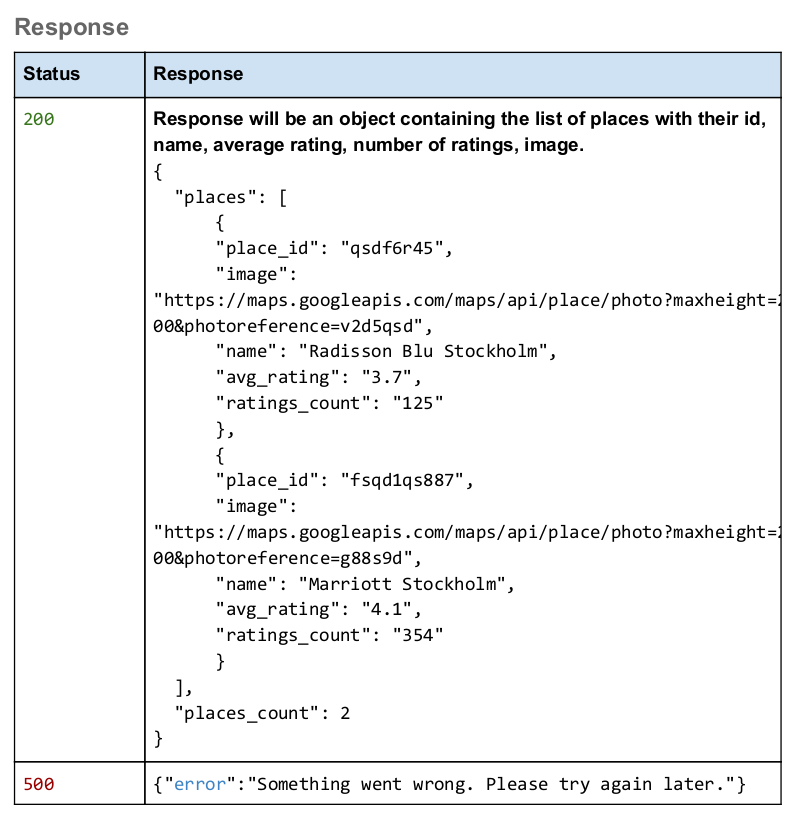
\includegraphics[width=15cm]{searchDocResponse.png}



\paragraph{Get place details}~\\
Get the details of a specific place using its place\_id

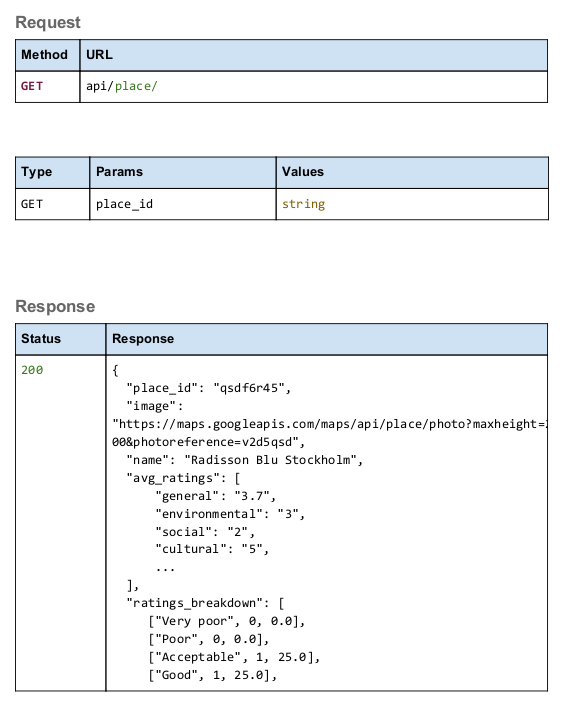
\includegraphics[width=15cm]{detailsDoc.png}

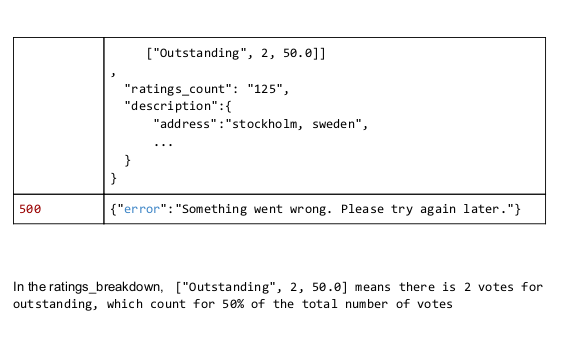
\includegraphics[width=15cm]{detailsDocResponse.png}



\paragraph{Get reviews}~\\
Get the reviews of a place using its place\_id

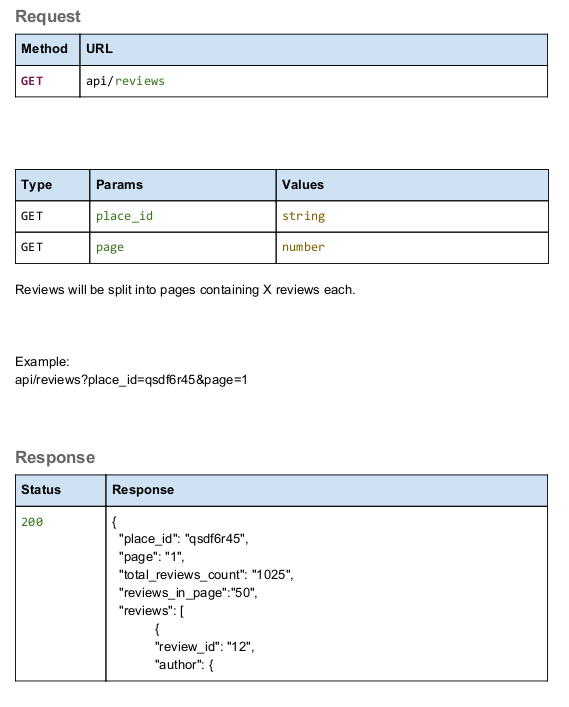
\includegraphics[width=15cm]{reviewsDoc.png}

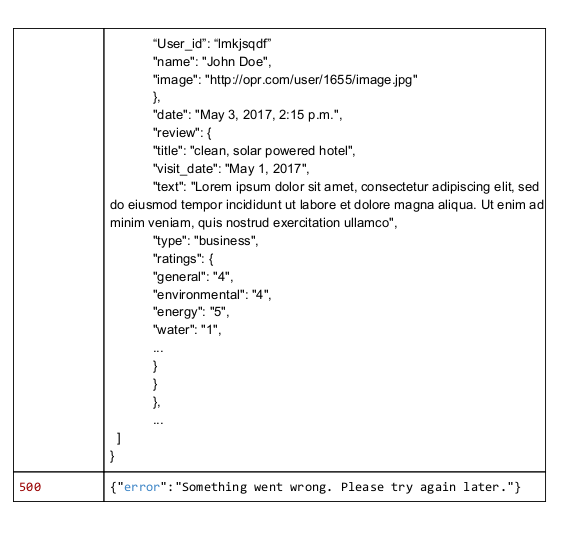
\includegraphics[width=15cm]{reviewsDocResponse.png}


\paragraph{Add review}~\\
Add a new review to a place

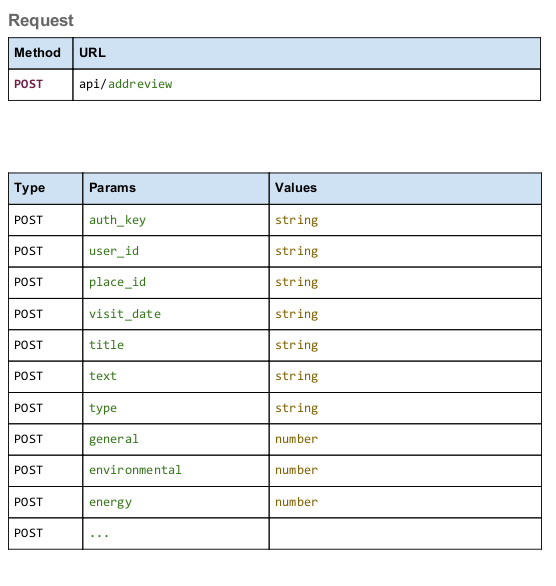
\includegraphics[width=15cm]{addDoc.png}

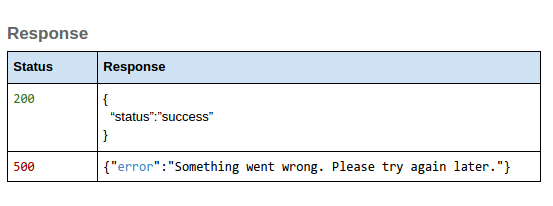
\includegraphics[width=15cm]{addDocResponse.png}


\chapter{Implementation}
\section{Technology choices}

\paragraph{Frontend}~\\
For the front-end I used HTML/CSS/JS with JQuery library because it facilitates basic
functionalities like DOM manipulation.\\
I also used twitter's Bootstrap in order to use its prebuilt components like the buttons.


\paragraph{Backend}~\\

The programming language used is Python, with the framework Django.\\
After careful thought I went with this choice because of several factors, including but not limited
to:
\begin{itemize}

\item Portability: this stack is cross-platform and can run on linux as well as windows
\item  Lots of tools out of the box: this choice offers:
\begin{itemize}

\item Runtime + Web framework
\item Package manager (PIP)
\item A database to test with (sqlite)
\item A lightweight development server
\item Unit testing library
\end{itemize}
\item Integrated ORM
\item Lots of libraries and ready-to-use components
\item  Abundant support and documentation
\item  Stability and reliability
\item  Scalability
\item  Great community
\end{itemize}

This boils down to creating a prototype quickly with this technology stack; we can get a lot done
in little time. Timing is a crucial part of this project, especially in this phase (prototyping).


\paragraph{Database}~\\

While comparing multiple databases, I ended up with two of the most popular databases to
compare between: MySQL and PostgreSQL.\\
The following table shows some differences of how things work in MySQL vs. in PostgreSQL.


\begin{table}[H]
\centering
\begin{tabular}{|l|l|l|}
\hline
                  & MySQL                                                                                                            & PostgreSQL                                                                                                                                                                                                      \\ \hline
CREATE INDEX      & \begin{tabular}[c]{@{}l@{}}Entire table is locked for\\ writes\end{tabular}                                      & \begin{tabular}[c]{@{}l@{}}Entire table is locked for\\ writes.But PSQL has \\"CREATE INDEX\\ CONCURRENTLY"\\that permits the creation of\\ index without locking the\\ entire table (but it is slower)\end{tabular} \\ \hline
Adding new column & \begin{tabular}[c]{@{}l@{}}Entire table data needs to be\\ rewritten\end{tabular}                                & Instantaneous                                                                                                                                                                                                   \\ \hline
Connection model  & \begin{tabular}[c]{@{}l@{}}One thread/connection:\\ Easy to create but hard to\\ monitor and manage\end{tabular} & \begin{tabular}[c]{@{}l@{}}One process/connection:\\ Easier to monitor and\\ manage\end{tabular}                                                                                                                \\ \hline
\end{tabular}
\caption{MySQL vs PostgreSQL}
\label{my-label}
\end{table}

I decided to use PostgreSQL as a database because of the previous comparison\cite{ANAND} and because
it is well supported by Django.\\
This choice is someway influenced by the previous choice.

\paragraph{Server}~\\

I used an Ubuntu 16.04 LTS Virtual Private Server for hosting the project.
Ubuntu has a great community and support, is reliable, and the Long Term Support (LTS)
version remains maintained for 5 years, so we won't have to worry about upgrading the system
for five years.\\
Ubuntu is based on Debian, which is one of the most stable Linux distributions ever.\\
The provider of the VPS is Amazon Web Service (AWS). I used AWS because it offers a free
tier during the first year of use, and because it has extensive capabilities beyond offering a
simple VPS. One of the capabilities that interested me the most is the ease of scaling and
setting up load balancers for the project.

\paragraph{Web Server}~\\
I had the choice between Apache HTTP Server and NGINX.\\
Both of them are great web servers and have great communities and support, and both of them
are open source as well.\\
I went with NGINX because it's better performance-wise and is becoming more and more popular, while Apache HTTP server's userbase is shrinking\cite{ALEXANDRA} (fig.\ref{fig:nginxvsapache}).

\begin{figure}[H]
\centering
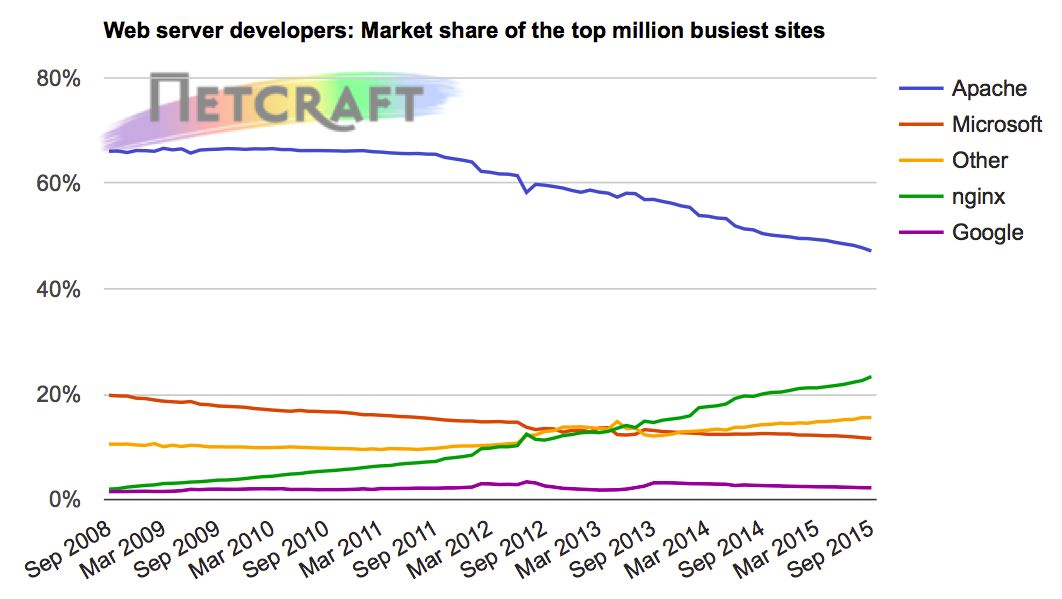
\includegraphics[width=15cm]{apache.png}
\caption{Chart showing how nginx's user base is growing while apache's is regressing}
\label{fig:nginxvsapache}
\end{figure}

\paragraph{Python Application server}~\\
I used Gunicorn as application server because it is the most popular and the best supported
server.
\paragraph{Additional Frameworks/libraries}

\subparagraph{Django-rest-framework}~\\
Django-rest-framework (DRF) supports the creation of REST APIs on top of Django.
This framework is django's standard tool to create REST APIs.

\subparagraph{Django-allauth}~\\
This is a library addressing authentication, registration, account management and social
authentication



\subparagraph{Django-rest-auth}~\\
This library makes the previously mentioned library (allauth) accessible via REST API




\subparagraph{Django-review}~\\
This is a library facilitating the creation of reviews and ratings. I found multiple libraries offering
reviews-related functionalities. I chose this library because it's kept updated and is backed by a
company.

\section{Screenshots}
\subsection{Web interface}

\begin{figure}[H]
\centering
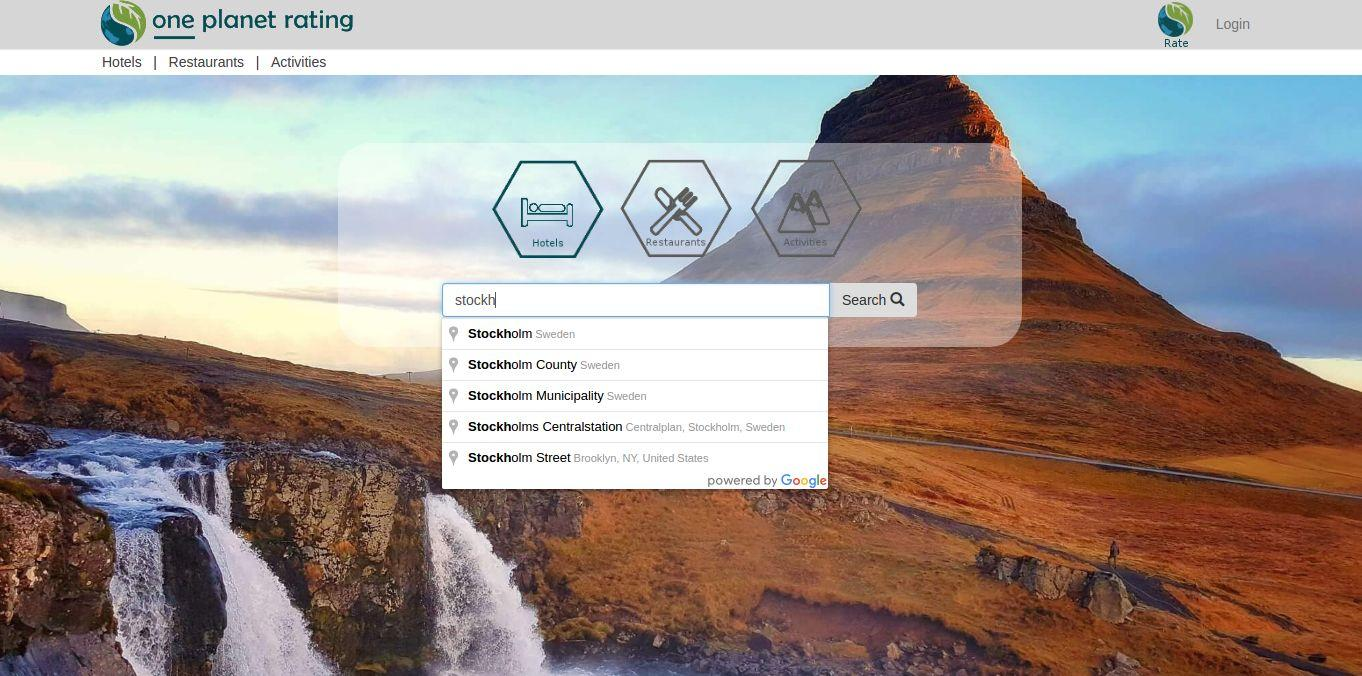
\includegraphics[width=15cm]{landing.jpg}
\caption{the landing screen of the app}
\label{screen:landing}
\end{figure}

When first accessed, the app shows the previous landing page (fig.\ref{screen:landing}). From there the user is able to
search for a place using the search bar.\\
The user is also to access the login screen from there.\\
Other functionalities include listing the popular and trending hotels using the links in the top left
corner, but these functionalities haven't been implemented yet.



\begin{figure}[H]
\centering
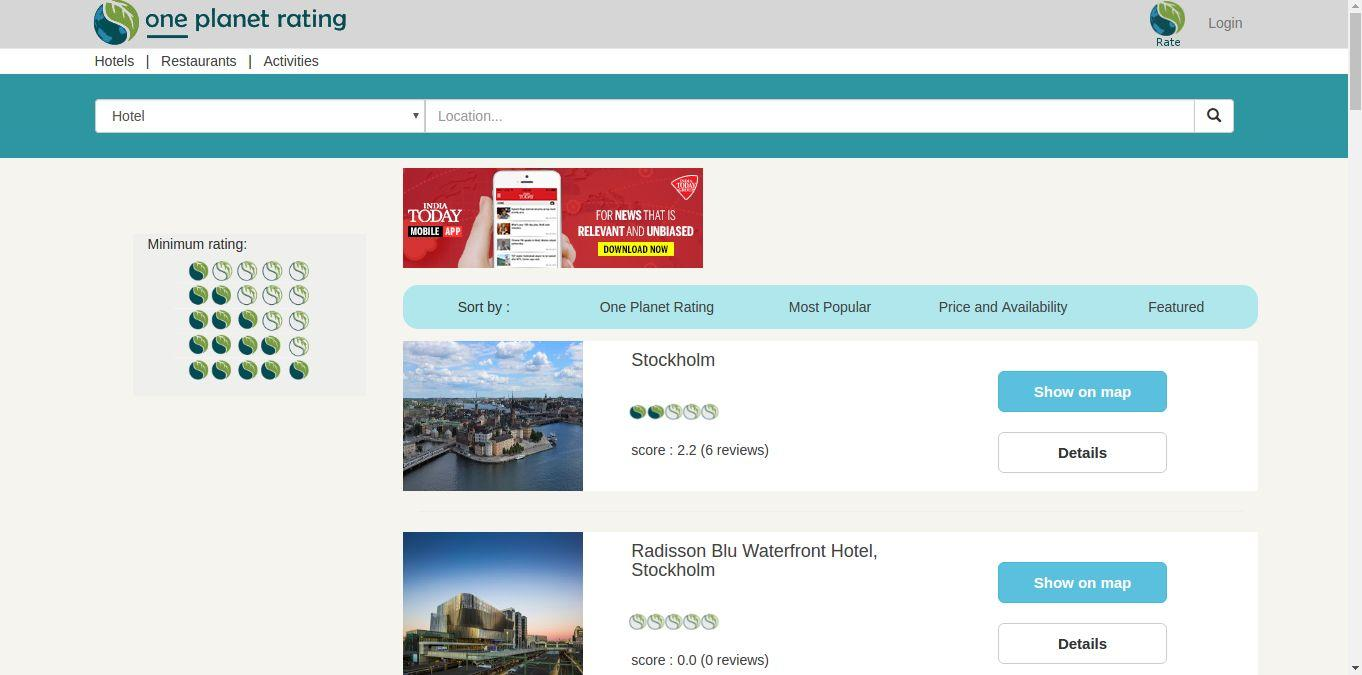
\includegraphics[width=15cm]{search.jpg}
\caption{search screen}
\label{screen:search}
\end{figure}

After the landing page, when a user searches for a place he will get redirected to this search
screen (fig.\ref{screen:search}) which includes the results retrieved from Google's places service. The search results
include the name and the picture (from google) as well as the number of reviews and the
average score from the reviews posted on OPR.




\begin{figure}[H]
\centering
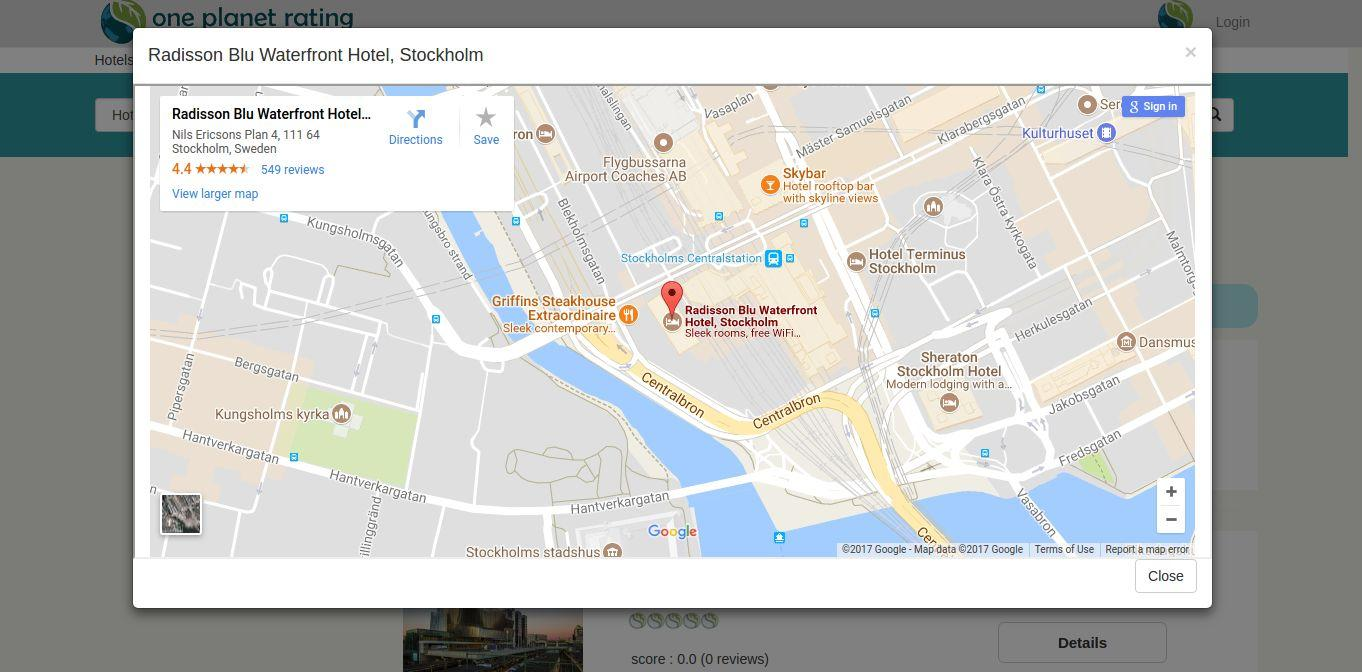
\includegraphics[width=15cm]{map.jpg}
\caption{showing the location of a place on the map}
\label{screen:map}
\end{figure}

From the search screen, the user is able to click the "show on map" button to see the selected
place on Google maps. The map is shown in a modal view (fig.\ref{screen:map}) in order for the user not to quit
OPR's site.




\begin{figure}[H]
\centering
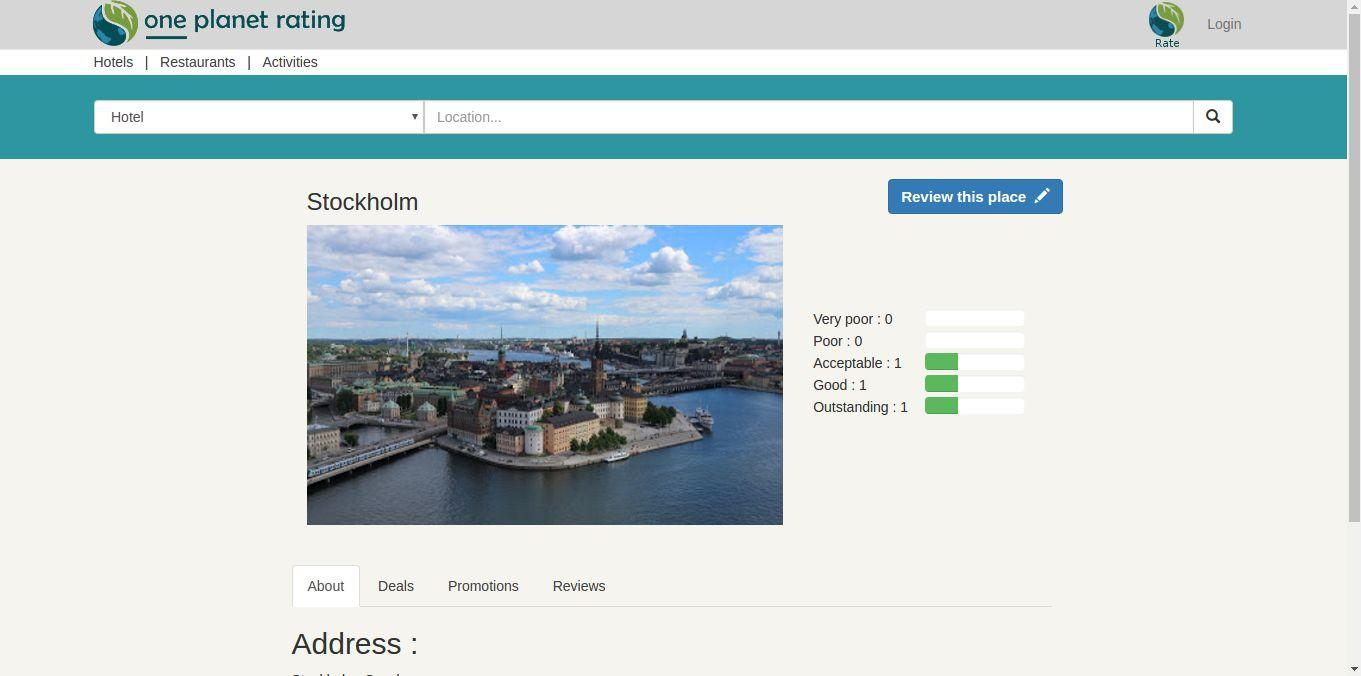
\includegraphics[width=15cm]{details.jpg}
\caption{place details}
\label{screen:details}
\end{figure}

When the user selects a place to see its details, he's shown this screen (fig.\ref{screen:details}); it contains the name,
picture and basic details of the place. This same screen also contains the reviews and a chart
showing the numbers and proportions of ratings.





\begin{figure}[H]
\centering
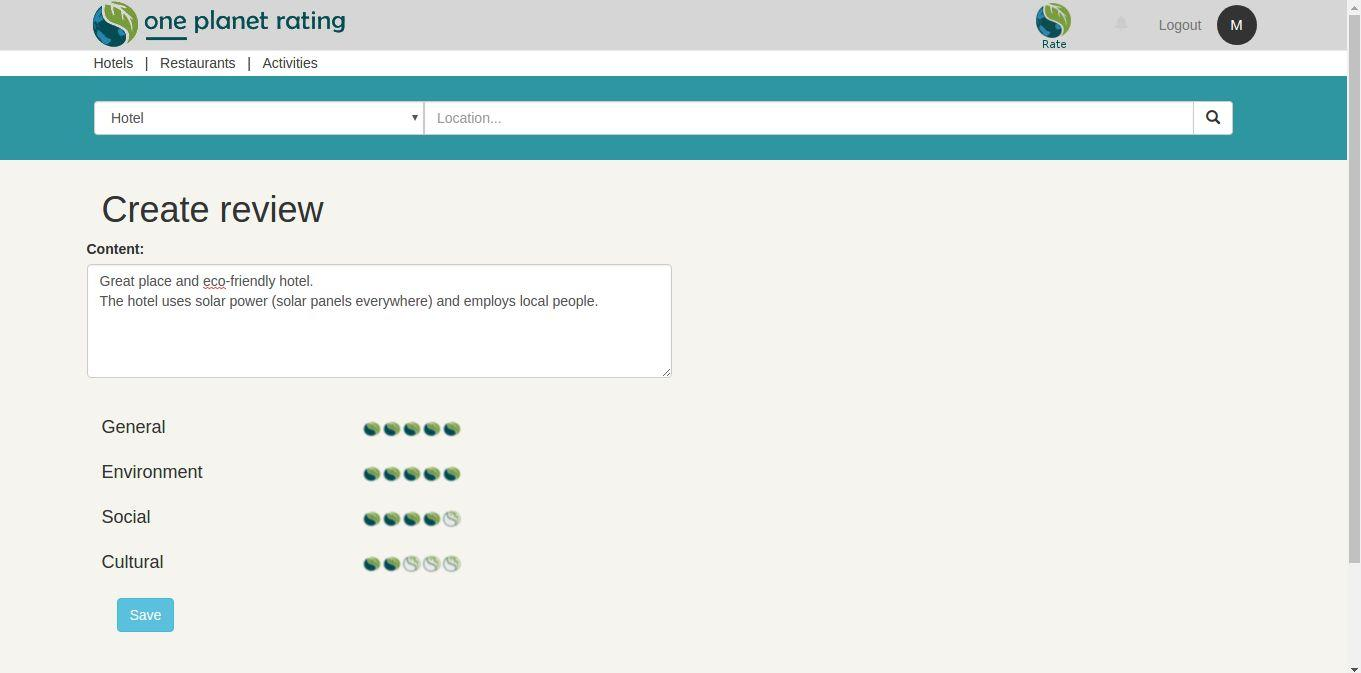
\includegraphics[width=15cm]{createReview.jpg}
\caption{Creating a review}
\label{screen:createreview}
\end{figure}


When the user chooses to create a review, the app first checks whether he's logged in.\\
If not, the user is redirected to the login screen, otherwise this form appears (fig.\ref{screen:createreview}). The form allows
the user to enter a text review as well as ratings following specific criteria.




\begin{figure}[H]
\centering
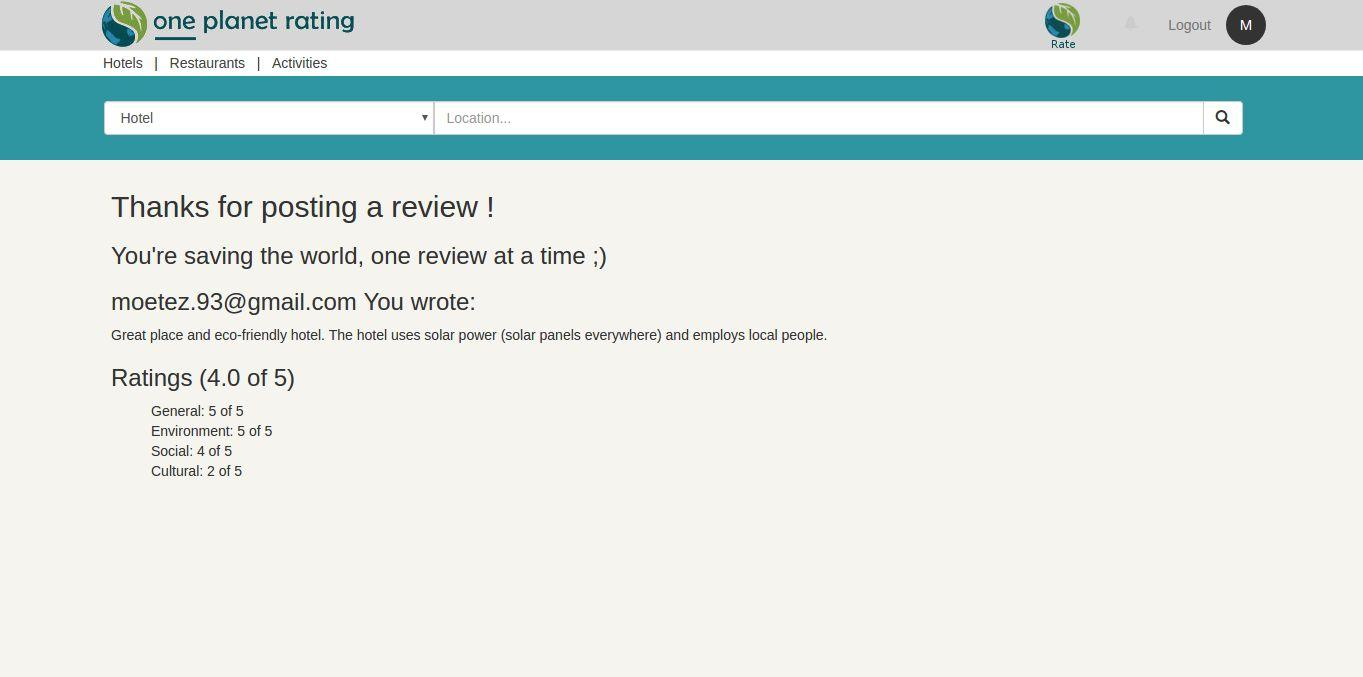
\includegraphics[width=15cm]{thanks.jpg}
\caption{Thanks screen}
\label{screen:thanks}
\end{figure}

After a member posts a review successfully, he's shown a thanks screen (fig.\ref{screen:thanks}).




\begin{figure}[H]
\centering
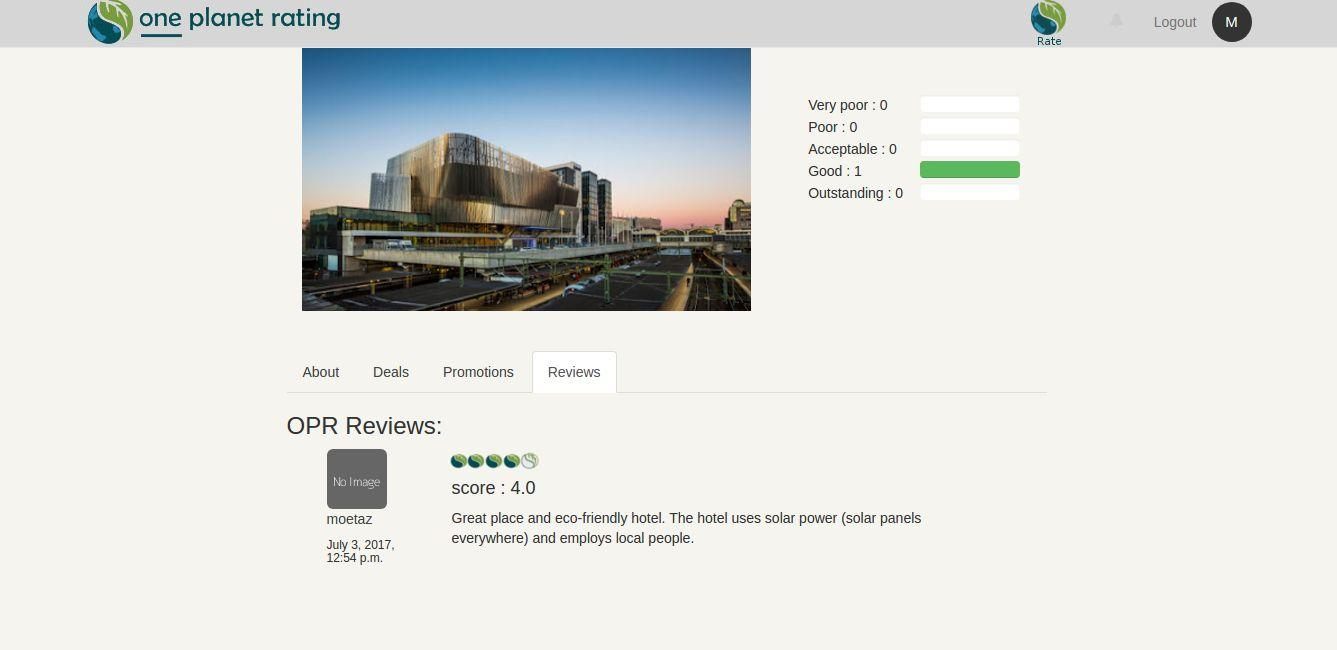
\includegraphics[width=15cm]{review.jpg}
\caption{Showing a review}
\label{screen:showreview}
\end{figure}

After a review is added, it is displayed as in this screenshot (fig.\ref{screen:showreview}). The score, text, username and date
are currently shown. Other features are being added like the user's photo and the categorized
ratings.

\subsection{API}



\begin{figure}[H]
\centering
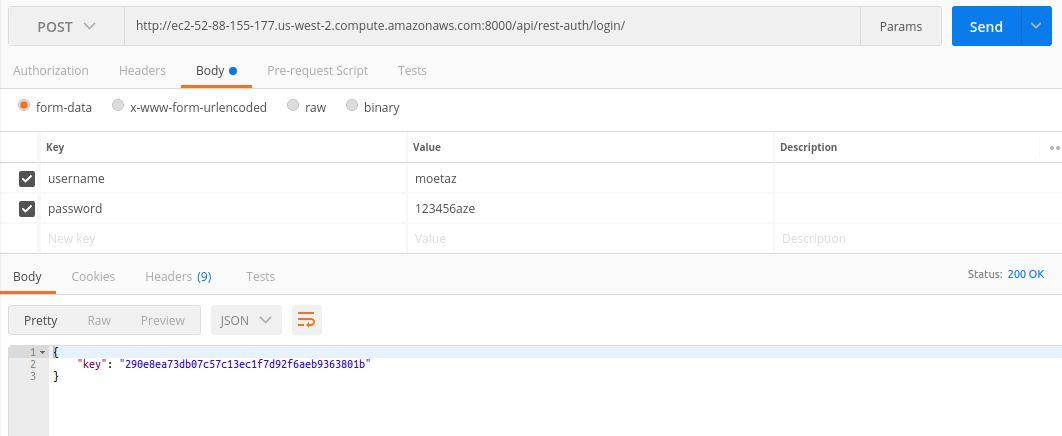
\includegraphics[width=15cm]{apilogin.jpg}
\caption{API Login}
\label{api:login}
\end{figure}

This screenshot (fig.\ref{api:login}) shows an example of a login request through the REST API.



\begin{figure}[H]
\centering
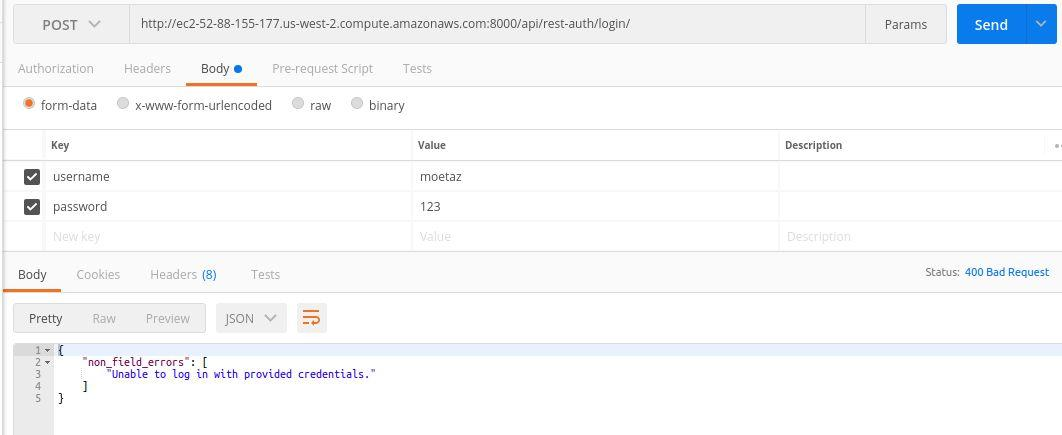
\includegraphics[width=15cm]{apiloginfail.jpg}
\caption{API Login failure}
\label{api:fail}
\end{figure}

In case of failure (wrong credentials), an error message is sent back to the user (fig.\ref{api:fail}).





\begin{figure}[H]
\centering
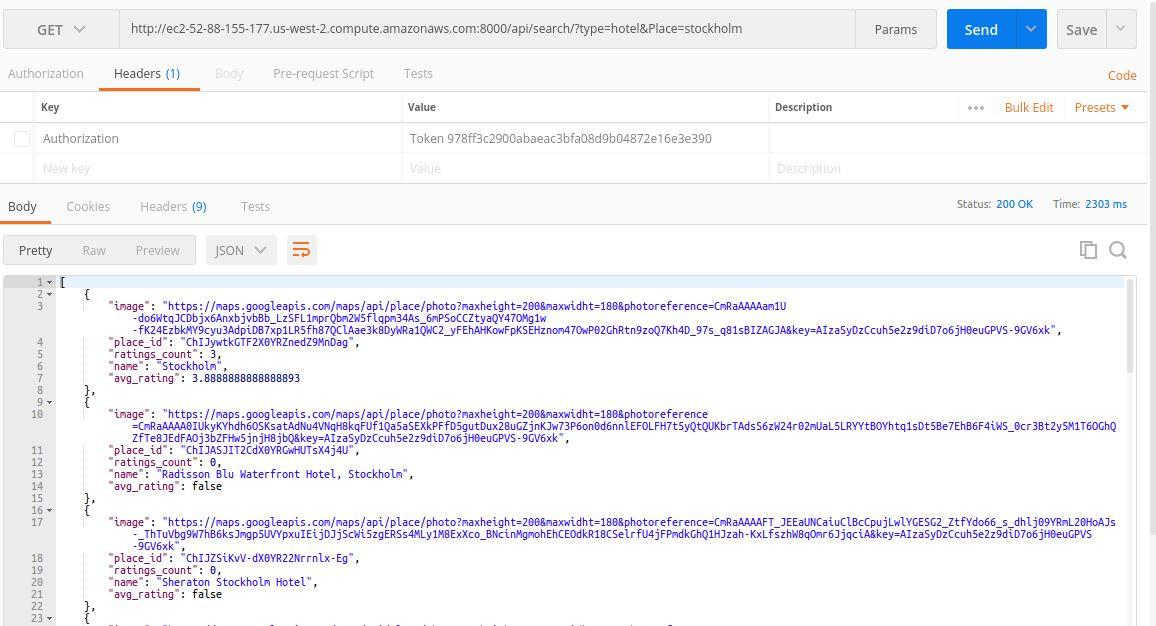
\includegraphics[width=15cm]{apisearch.jpg}
\caption{API search request}
\label{api:search}
\end{figure}

This screenshot (fig.\ref{api:search}) shows the response to a search query. The query includes as parameters the
type of place (hotel, restaurant..) as well as a keyword to specify the location.\\
The response contains the name, image, place\_id, ratings count , and the average rating.\\
The name and image are displayed as is. The ratings count and the average rating, however,
are used to display the globes/stars next to each place in the results list. The place\_id is used to
get the place's map or the place's details.






\begin{figure}[H]
\centering
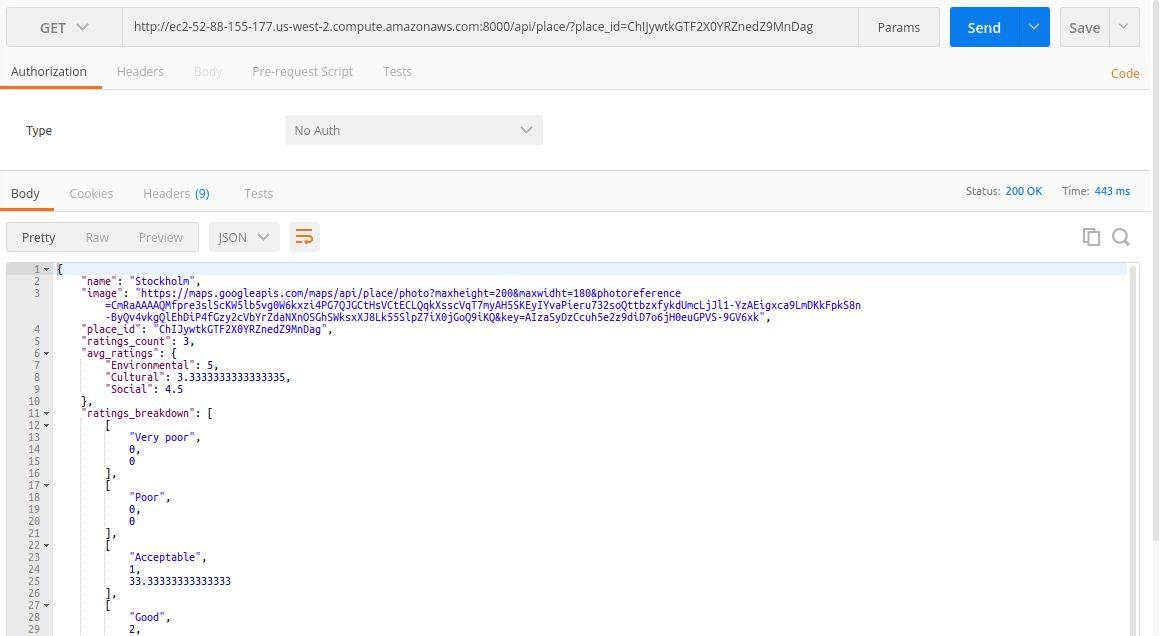
\includegraphics[width=15cm]{apidetails.jpg}
\caption{API place details}
\label{api:details}
\end{figure}

When requesting the details of a place (fig.\ref{api:details}), the request includes the place\_id of the place.\\
Obviously the response includes the name and image of the place, it also includes the number
and averages of ratings. It also contains the ratings breakdown, which consists of the
proportions of the ratings arranged by the number of stars ( 0 star = very poor, 1 star = poor...)





\begin{figure}[H]
\centering
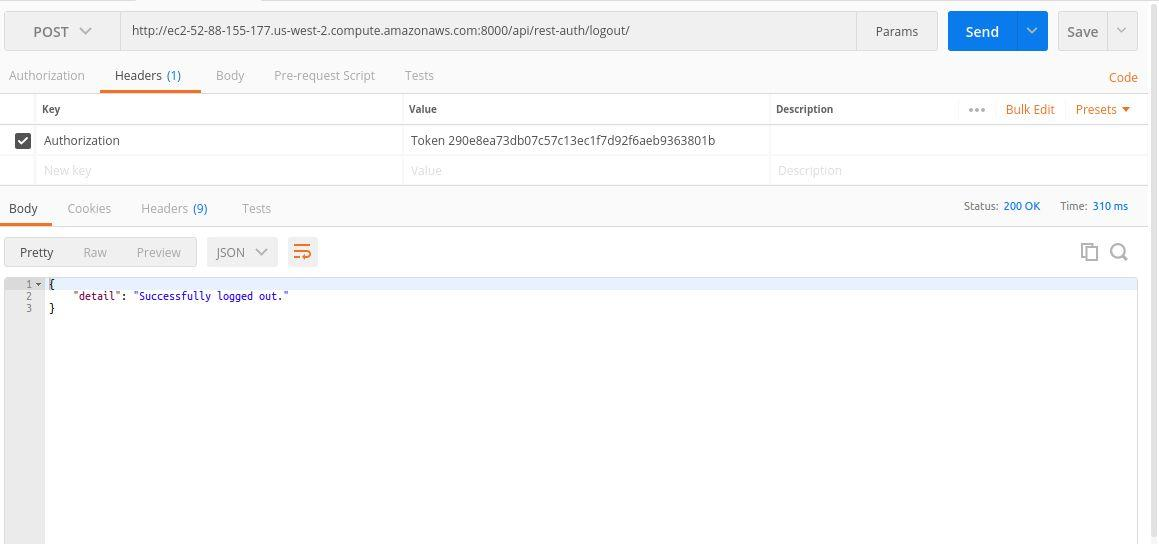
\includegraphics[width=15cm]{apilogout.jpg}
\caption{Logout API call}
\label{api:logout}
\end{figure}

This screenshot (fig.\ref{api:logout}) shows a successful logout call. The authentication is based on an authorization
token stored in the DB. After logging out, that token is deleted.

\section{Deployment}

\paragraph{AWS EC2 Security setup}~\\



\begin{figure}[H]
\centering
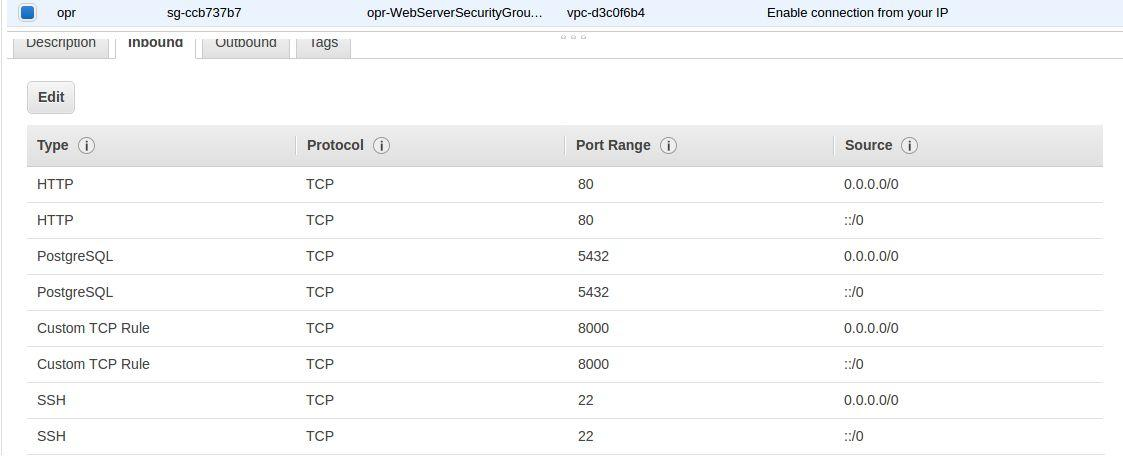
\includegraphics[width=15cm]{ec21.jpg}
\caption{AWS EC2 allowed inbound traffic}
\label{ec2:inbound}
\end{figure}


\begin{figure}[H]
\centering
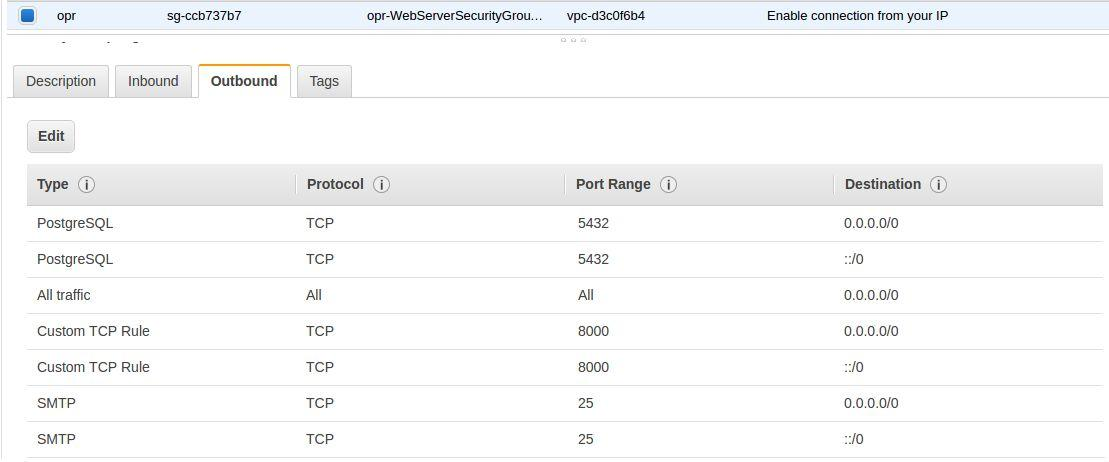
\includegraphics[width=15cm]{ec22.jpg}
\caption{AWS EC2 allowed outbound traffic}
\label{ec2:outbound}
\end{figure}

A problem I encountered during the deployment is to get the server to reply for requests.
In the beginning I was even unable to ssh into the VPS. It turned out, for security reasons AWS
blocks all incoming\cite{EC2DOC} (fig.\ref{ec2:inbound}) and outgoing (fig.\ref{ec2:outbound}) traffic.


\paragraph{AWS RDS setup}~\\


\begin{figure}[H]
\centering
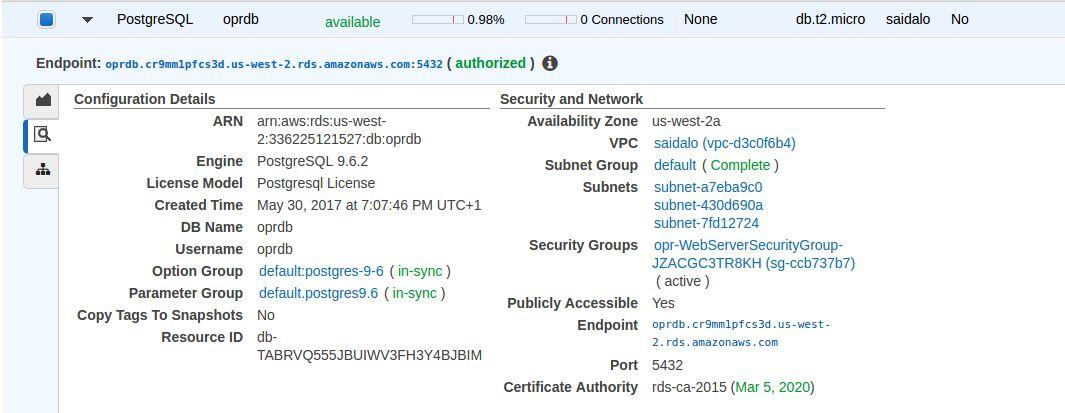
\includegraphics[width=15cm]{rds.jpg}
\caption{AWS RDS setup}
\label{rds}
\end{figure}

I used AWS RDS (fig.\ref{rds}) for hosting the database because security wise it's better approach to host the
database separately from the app. Another advantage of AWS RDS is that it automatically
creates backups of the DB\cite{RDSDOC}.\\
First I hosted a local db for testing purposes then I moved the same DB to RDS.


\paragraph{NGINX setup}~\\


NGINX is the entrypoint to the app. It's also the web server used to serve the app. NGINX was
setup to listen on port 8000 and to serve the static files like the images and css ( practically
every url pointing to /static). In case of non static files, NGINX redirects the request to gunicorn
which is the python server that's serving the app. For the configuration of NGINX please refer to "NGINX configuration" in the appendix

\section{Testing}

For the development of searchAd module, which is a sort of standalone library, I also created
unit tests (fig.\ref{unittest}) for it.\\
The unit tests ensure that the code works correctly, and helps verify that the code didn't break
after some changes. This provides better quality and saves more time.


\begin{figure}[H]
\centering
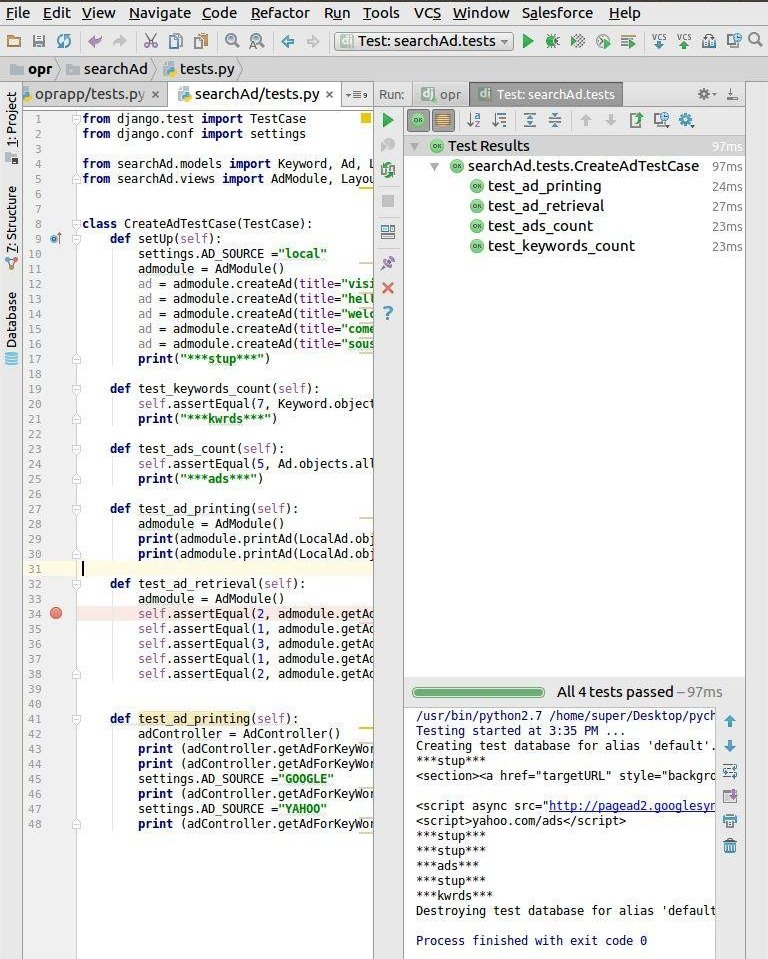
\includegraphics[width=13cm]{unittests.jpg}
\caption{unit tests}
\label{unittest}
\end{figure}


I also tested the performance of the app (load speed) using google's Pagespeed Insights, and I
got some amazing results (fig. \ref{speed1} and fig.\ref{speed2})




\begin{figure}[H]
\centering
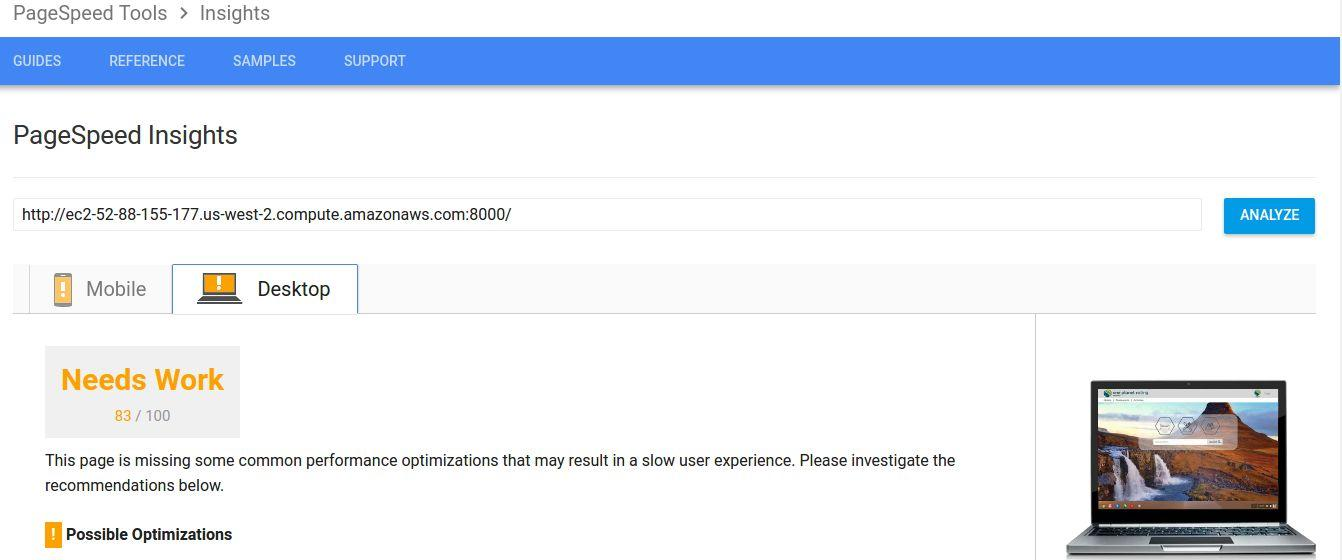
\includegraphics[width=15cm]{speed1.jpg}
\caption{landing page speed test}
\label{speed1}
\end{figure}



\begin{figure}[H]
\centering
\includegraphics[width=15cm]{speed2.jpg}
\caption{details page speed test}
\label{speed2}
\end{figure}

Below (fig.\ref{speed3}) is included the result for the same test applied to facebook.com for comparison purposes:





\begin{figure}[H]
\centering
\includegraphics[width=15cm]{fbtest.jpg}
\caption{facebook page speed test}
\label{speed3}
\end{figure}


I also tested the performance of the app using blazemeter (fig.\ref{blaze}). I tested the service with 50
simultaneous virtual users and the results were good enough.




\begin{figure}[H]
\centering
\includegraphics[width=15cm]{blaze.jpg}
\caption{concurrent users test}
\label{blaze}
\end{figure}

With 50 simultaneous users the response time was ~170ms which is okay. Note that the
performance is influenced by the performance amazon's server, which is very limited but easily
scalable. For the development, I went with a low-performance server instance because of
budgetary reasons, but we can scale up easily later when we need to.
The used instance is an AWS EC2 t2.micro with the following specs:
\begin{itemize}
\item RAM: 1 GB
\item vCPUs: 1
\end{itemize}

\section{Work environment}
All of the development was made on my personal laptop which has the following specs:
\begin{itemize}
\item RAM: 8GB
\item CPU: Intel core i7
\item OS: Ubuntu 16.04 LTS
\end{itemize}

\paragraph{PyCharm}~\\
During the development I used the IDE PyCharm. It's developed by JetBrains, the world leader in IDEs development. PyCharm's user interface is very user-friendly and familiar because it's similar to the company's other products.\\
PyCharm is also extremely powerful. To name a few of its features we can cite: code completion, debugging and integrated version control tools.

\paragraph{BitBucket}~\\
For version control we used Git, hosted on BitBucket. Git is the most popular distributed version control system. It's widely used and very powerful. It allows developers to keep all the history of the project, and allows them to collaborate efficiently. BitBucket offers unlimited free private git repositories for teams of up to 5 people.
\paragraph{Slack}~\\
Communication was all held on Slack. Slack is becoming the standard in the corporate communication tools and is used by some of the biggest organizations in the world like NASA. Slack allows people to create chat channels, share files, and hold audio and video calls from the web browser. Another major powerful feature of Slack is that it has multiple plugins and external integrations.
\paragraph{draw.io \& Dia}~\\
The diagrams were made using Dia and draw.io\\Both of these tools are open source and very popular.
The main difference is that Dia runs locally while draw.io runs on the browser. Both of these tools are powerful, versatile and have ready-to-use UML components.
~\\
\paragraph{GIMP}~\\
In the beginning of the project I also did some graphic design using GIMP, which is an open
source and free alternative to photoshop.\\ GIMP allows the creation of layers, transparency, filters and many advanced features that were very useful during the design phase.
\paragraph{InvisionApp}~\\
I used InvisionApp to create an interactive prototype using the mockups I designed.\\ InvisionApp allows the creation of prototypes from images only. Images become clickable and the behaviour is customizable. The prototype can then be tested in the browser or using a mobile device, and gives a very real experience.
\paragraph{Chrome developer tools}~\\
Chrome developer tools were used extensively for debugging and tweaking the frontend.\\The tools offer several features from simple ones like changing the styling of the DOM and seeing the changes in realtime to more advanced operations like debugging JavaScript code in the browser and monitoring the requests and their responses.
\paragraph{Postman}
Postman was used to test the REST requests for the API.\\ Postman is a Chrome extension that allows to send custom HTTP requests and preview their responses. In the beginning I used curl, but it turned out Postman is a lot more efficient.
\paragraph{Unittest}
Unittest is a python library for unit testing. It's included with python by default. I used it for testing the searchAd module.



\chapter{Conclusion}

The work done during my internship constitutes the first working prototype of OPR.
In the beginning a substantial effort and time was dedicated to analyze the project and identify the available alternatives. We also defined the specification and requirements in details so we can have a clear vision about the needs that the project should satisfy.\\
Then we went through the design aspects and set the physical architecture (we chose AWS' EC2 and RDS with NGINX as a web server, Gunicorn as python server, PostgreSQL as DB and Ubuntu LTS as OS). We also went through the logical architecture and we decided to use MVC + 3 Tiers. The last step in the design process was to set the modular architecture of the project.\\
Finally we covered the implementation details, by explaining the tool choices and tech stack as well as exposing how the system works. We also covered the deployment process, configuration and the tests that the project went through.\\~\\
The prototype is being tested internally and soon to be released to the public. 
But before becoming production ready, the app needs security and penetration testing.
Also, now that the project is getting bigger, the project should also take advantage of more sophisticated yet facilitating tools, like continuous integration, continuous deployment and containerization.\\~\\
The REST API might also turn out useful if the frontend of the web app gets redesigned using a single-page app framework such as React or Angular.
Other performance improvements can be easily implemented, like using a Content Delivery Network to deliver the static files, but the project is still not big enough and not mature enough to require such optimizations.\\~\\
The project is easily scalable, especially with the help of AWS which allows the expansion of the infrastructure in a couple of clicks\cite{EC2DOC}\cite{RDSDOC}. During the deployement I set up a couple instances and a loadbalancer to test the high-availability of the service and it worked perfectly, but I later removed it for budgetary reasons.




\begin{thebibliography}{9}

\bibitem{PAOLO} 
Paolo Anania. \\
\textit{Arbeiten bei Trivago: Keine Hierarchien und 15 Biersorten gratis}. (German) \\
\textit{Working with Trivago: No hierarchy and 15 offices}. (English) \\
\href{http://www.lead-digital.de/aktuell/work/arbeiten_bei_trivago_keine_hierarchien_und_15_biersorten_gratis}{http://www.lead-digital.de/aktuell/work/arbeiten\_bei\_trivago\\\_keine\_hierarchien\_und\_15\_biersorten\_gratis}.



\bibitem{WERNER}
Werner Vogels, CTO@Amazon\\
\textit{Working Backwards}\\
\href{http://www.allthingsdistributed.com/2006/11/working_backwards.html}{http://www.allthingsdistributed.com/2006/11/working\_backwards.html}.


\bibitem{ANAND} 
Anand Chitipothu. \\
\textit{Ten Reasons Why You Should Prefer PostgreSQL to MySQL
}. \\
\href{https://www.slideshare.net/anandology/ten-reasons-to-prefer-postgresql-to-mysql}
{https://www.slideshare.net/anandology/ten-reasons-to-prefer-postgresql-to-mysql}.



\bibitem{JUSTIN} 
Justin Ellingwood. \\
\textit{How To Set Up Django with Postgres, Nginx, and Gunicorn on Ubuntu 16.04
}. \\
\href{https://www.digitalocean.com/community/tutorials/how-to-set-up-django-with-postgres-nginx-and-gunicorn-on-ubuntu-16-04}
{https://www.digitalocean.com/community/tutorials/how-to-set-up-django-with-postgres-nginx-and-gunicorn-on-ubuntu-16-04}.


\bibitem{ALEXANDRA} 
Alexandra Leslie. \\
\textit{NGINX vs. Apache (Pro/Con Review, Uses, \& Hosting for Each)
}. \\
\href{http://www.hostingadvice.com/how-to/nginx-vs-apache/}
{http://www.hostingadvice.com/how-to/nginx-vs-apache/}.



\bibitem{RDSDOC} 
Amazon web services. \\
\textit{AWS RDS Documentation
}. \\
\href{http://docs.aws.amazon.com/AmazonRDS/latest/UserGuide/Welcome.html}
{http://docs.aws.amazon.com/AmazonRDS/latest/UserGuide/Welcome.html}.


\bibitem{EC2DOC} 
Amazon web services. \\
\textit{AWS EC2 Documentation
}. \\
\href{http://docs.aws.amazon.com/AWSEC2/latest/UserGuide/concepts.html}
{http://docs.aws.amazon.com/AWSEC2/latest/UserGuide/concepts.html}.


\bibitem{UNESCO} 
 John Fien, Margaret Calder and Clayton White. \\
\textit{Sustainable tourism
}. \\
\href{http://www.unesco.org/education/tlsf/mods/theme_c/mod16.html}
{http://www.unesco.org/education/tlsf/mods/theme\_c/mod16.html}.



\bibitem{UN} 
 United Nationas. \\
\textit{Sustainable Development Goals
}. \\
\href{https://sustainabledevelopment.un.org/sdgs}
{https://sustainabledevelopment.un.org/sdgs}.


\end{thebibliography}

\chapter*{Appendix}
\section{NGINX configuration}
\includegraphics[width=15cm]{nginx.jpg}

\end{document}
